\documentclass{article} % For LaTeX2e
\usepackage[final]{colm2026_conference}

\usepackage{microtype}
\usepackage{hyperref}
\usepackage{url}
\usepackage{booktabs}
\usepackage[draft]{graphicx}
\usepackage{amsmath}
\usepackage{enumitem}
\usepackage{multirow}
\usepackage{algorithm}
\usepackage{algorithmic}
\usepackage{float}

\usepackage{lineno}

% Allow more floats per page
\renewcommand{\topfraction}{0.95}
\renewcommand{\bottomfraction}{0.95}
\renewcommand{\textfraction}{0.05}
\renewcommand{\floatpagefraction}{0.9}
\setcounter{topnumber}{6}
\setcounter{bottomnumber}{4}
\setcounter{totalnumber}{10}

\definecolor{darkblue}{rgb}{0, 0, 0.5}
\hypersetup{colorlinks=true, citecolor=darkblue, linkcolor=darkblue, urlcolor=darkblue}


\title{Hybrid Pragmatic-Structural Reasoning with Group Relative\\Policy Optimization for Sarcasm Detection}

\author{
  Luo Wentao \And Zhao Xun \And Yan Zihao
}

\graphicspath{{Figure/}}

\begin{document}

\ifcolmsubmission
\linenumbers
\fi

\maketitle

\begin{abstract}
Sarcasm detection remains a challenging task in natural language understanding due to the subtle gap between literal wording and intended meaning. In this work, we conduct a systematic study comparing four approaches built on the same large language model: (1) direct classification, (2) Pragmatic Metacognitive Prompting (PMP), (3) Rhetoric-Context-Emotion (RCE) structured reasoning with Group Relative Policy Optimization (GRPO), and (4) a novel hybrid framework that unifies PMP and RCE reasoning within a single GRPO training procedure using multi-component rewards. Experiments on SemEval 2018 Task 3 show that the hybrid framework achieves the best performance across both a 200-sample subset (75.0\% accuracy, 75.0 Macro-F1) and the full 784-sample test set (69.5\% accuracy, 69.3 Macro-F1). Analysis reveals that combining pragmatic incongruity analysis with structured linguistic reasoning significantly reduces false positives while maintaining high sarcastic recall.
\end{abstract}

\section{Introduction}

Sarcasm is a form of verbal irony in which the intended meaning differs from the literal expression, often used to convey criticism, mockery, or humor. Detecting sarcasm in text is a long-standing challenge in natural language processing (NLP), as it requires understanding pragmatic incongruity, speaker intent, contextual knowledge, and emotional subtext~\citep{joshi2017context}. Traditional approaches based on lexical features, sentiment analysis, or supervised classifiers struggle with the nuanced and context-dependent nature of sarcastic language.

Recent advances in large language models (LLMs) have opened new possibilities for sarcasm detection. Rather than relying solely on surface-level features, LLMs can reason about the pragmatic aspects of text through carefully designed prompts. Two prominent directions have emerged: (1) prompting-based approaches that guide the model to analyze pragmatic incongruity, and (2) structured reasoning approaches that decompose sarcasm evidence into interpretable dimensions.

\citet{pmp} proposed Pragmatic Metacognitive Prompting (PMP), which leverages principles from pragmatics and metacognition to help LLMs interpret implied meanings, consider contextual cues, and reflect on discrepancies. Separately, \citet{sarcasmr1} introduced a three-dimensional reasoning framework based on Rhetoric, Context, and Emotion (RCE) signals, combined with Group Relative Policy Optimization (GRPO)~\citep{deepseekr1} to reinforce desired reasoning behaviors.

These two approaches capture complementary aspects of sarcasm. PMP focuses on the pragmatic gap between literal and intended meaning, while RCE provides structured linguistic evidence. We hypothesize that combining both reasoning paradigms within a unified GRPO training framework can lead to better sarcasm detection by leveraging a more comprehensive set of cues.

Our main contributions are:
\begin{enumerate}[leftmargin=*, itemsep=0pt]
    \item A systematic comparison of four sarcasm detection approaches---direct classification, PMP prompting, RCE reasoning with GRPO, and a hybrid PMP-RCE approach with GRPO---all using the same base model (Qwen3-14B) to isolate the effect of reasoning strategies.
    \item A novel hybrid framework that integrates pragmatic metacognitive analysis with structured RCE reasoning in a three-phase prompt, optimized by a multi-component GRPO reward function.
    \item Comprehensive evaluation on SemEval 2018 Task 3 with detailed analysis showing that the hybrid approach achieves the best balance between sarcastic recall and non-sarcastic precision.
\end{enumerate}

Figure~\ref{fig:overview} provides an overview of the four frameworks examined in this study.

\begin{figure}[htbp]
\begin{center}
\includegraphics[width=\linewidth]{pipeline_overview.png}
\end{center}
\caption{Overview of the four sarcasm detection frameworks. All share the same Qwen3-14B backbone. The Baseline uses direct classification; FW1 applies PMP prompting without training; FW2 combines RCE reasoning with GRPO; FW3 unifies PMP and RCE in a hybrid prompt optimized by multi-component GRPO rewards.}
\label{fig:overview}
\end{figure}


\section{Related Work}

\paragraph{Sarcasm Detection.}
Early work on sarcasm detection relied on handcrafted features such as sentiment incongruity, punctuation patterns, and lexical cues~\citep{joshi2017context}. With the rise of deep learning, neural models based on LSTMs, attention mechanisms, and pre-trained transformers improved performance by capturing contextual representations. However, these models often treat sarcasm detection as a standard text classification task without explicitly modeling the reasoning behind sarcastic interpretations.

\paragraph{Prompting and Reasoning with LLMs.}
Chain-of-thought prompting~\citep{wei2022chain} demonstrated that guiding LLMs to produce intermediate reasoning steps improves performance on complex tasks. In sarcasm detection, \citet{pmp} applied pragmatic metacognitive prompting to encourage models to analyze implicature, presupposition, and speaker intent before making a decision. Their approach showed improvements over direct classification, particularly in reducing false positives caused by over-predicting sarcasm from negative sentiment alone.

\paragraph{Reinforcement Learning for LLMs.}
Reinforcement learning from human feedback (RLHF)~\citep{ouyang2022training} has been widely adopted to align LLMs with desired behaviors. \citet{deepseekr1} introduced Group Relative Policy Optimization (GRPO), a simpler alternative that replaces the critic network with group-relative advantage estimation. GRPO has been successfully applied to mathematical reasoning and code generation. \citet{sarcasmr1} adapted GRPO for sarcasm detection by designing multi-component reward functions that encourage structured reasoning alongside classification accuracy.

\paragraph{Structured Sarcasm Reasoning.}
\citet{sarcasmr1} proposed decomposing sarcasm evidence into three dimensions: Rhetoric (irony, hyperbole, contrast), Context (situational mismatch, common sense violation), and Emotion (sentiment gap, emotional reversal). Their reward function incentivizes the model to reason across all three dimensions before producing a final classification. Our work extends this line by integrating RCE reasoning with PMP-style pragmatic analysis.


\section{Method}

\subsection{Task Formulation}

Given a text $x$, the goal is to predict a binary label $y \in \{\texttt{sarcastic}, \texttt{non\_sarcastic}\}$. All four methods described below use the same base model Qwen3-14B, ensuring that performance differences arise from the reasoning strategy rather than model capability.

\subsection{Baseline: Direct Classification}

The baseline prompts the model with a simple instruction to classify the text as sarcastic or non-sarcastic without any intermediate reasoning. The prompt asks the model to output only a final label in the format \texttt{[Final] \{label\}}. This establishes a lower bound that reflects the model's native sarcasm detection ability.

\subsection{Framework~1: Pragmatic Metacognitive Prompting}

Framework~1 adopts the PMP approach~\citep{pmp} with a two-phase reasoning prompt:

\paragraph{Phase 1: Preliminary Pragmatic Analysis.}
The model analyzes six pragmatic dimensions: (1) \textit{implicature}---what is implied beyond the literal wording; (2) \textit{presupposition}---what background assumptions the text relies on; (3) \textit{speaker intent}---what the speaker appears to be trying to achieve; (4) \textit{polarity}---whether the surface tone is positive, negative, or neutral; (5) \textit{pretense}---whether the speaker is pretending to hold an attitude they likely do not hold; and (6) \textit{meaning gap}---whether there is a clear difference between literal and implied meaning. These factors are motivated by pragmatic theories of non-literal meaning, especially the idea that speakers can communicate more than they literally say through implicature and contextual inference~\citep{grice1975}.

\paragraph{Phase 2: Reflection and Calibration.}
The model reassesses the pragmatic analysis, identifies evidence for and against sarcasm, and applies calibration rules to avoid over-predicting sarcasm from negative emotion alone. A key decision rule requires clear pragmatic incongruity---the speaker's implied attitude must conflict with the literal wording or involve pretense.

\paragraph{Two-Call vs.\ Full PMP.}
We implement two variants. \textit{PMP two-call} separates analysis and reflection into two model invocations: the first call $a = M(P_1(x, c))$ generates a preliminary pragmatic analysis, and the second call $y = M(P_2(x, c, a))$ reflects on this analysis and produces the final label. \textit{Full PMP} compresses both stages into a single prompt, asking the model to analyze, reflect, and answer in one generation. Full PMP avoids cross-turn drift and proves more effective in practice.

\paragraph{Compared Prompting Strategies.}
To isolate the effect of pragmatic structure, we also test seven other prompt designs on the same evaluation pipeline: Input-Output (IO) direct prompting, simple baseline, Chain-of-Thought (CoT)~\citep{wei2022chain}, Tree-of-Thought (ToT)~\citep{yao2023tot}, Bag-of-Clues (BoC), Chain-of-Clues (CoC), and Graph-of-Clues (GoC). These clue-based prompts test whether explicit cue extraction can compete with the pragmatic factors in PMP. All strategies are run through the same experimental runner controlling for data split, decoding, and metric computation.

Framework~1 does not involve any parameter training; it relies entirely on prompting. Figure~\ref{fig:fw1} illustrates the PMP prompt structure.

\begin{figure}[htbp]
\begin{center}
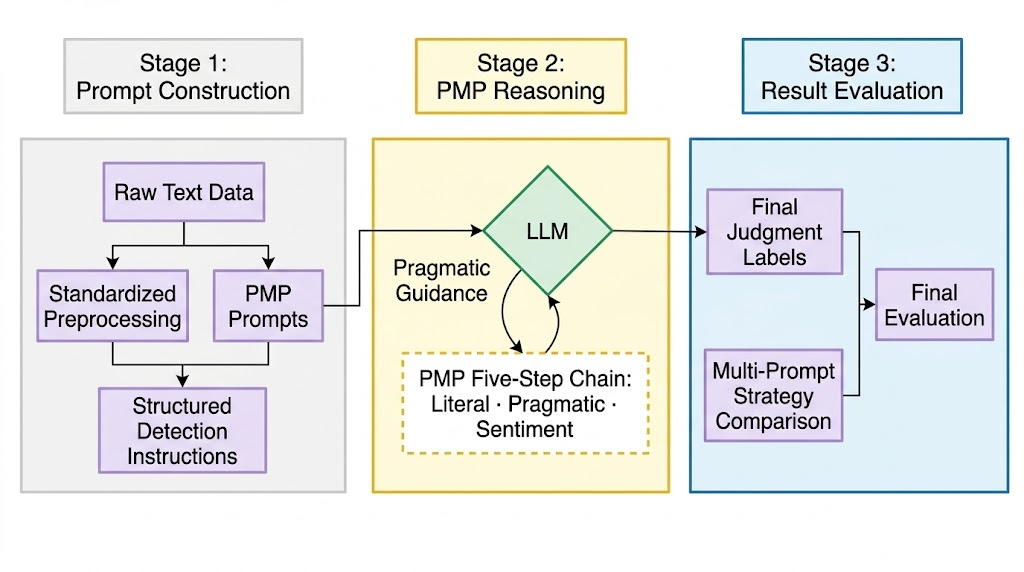
\includegraphics[width=\linewidth]{framework_one.png}
\end{center}
\caption{Framework~1 (PMP): two-phase pragmatic metacognitive prompting. Phase~1 analyzes six pragmatic dimensions; Phase~2 reflects and calibrates before producing the final label.}
\label{fig:fw1}
\end{figure}

\subsection{Framework~2: RCE Reasoning with GRPO}

Framework~2 builds on the Sarcasm-R1 approach~\citep{sarcasmr1} by introducing structured reasoning over three dimensions and training the model with GRPO.

\paragraph{Three-Dimensional Reasoning.}
The model analyzes sarcasm evidence along three axes:
\begin{itemize}[leftmargin=*, itemsep=0pt]
    \item \textbf{Rhetoric}: irony, hyperbole, understatement, mock praise, contrast, quotation marks, hashtags, and other rhetorical signals.
    \item \textbf{Context}: whether the literal statement fits the situation, common sense, or background knowledge, or creates a contextual contradiction.
    \item \textbf{Emotion}: comparison between surface emotion and implied emotion, looking for emotional mismatch such as positive wording with negative intent.
\end{itemize}

\paragraph{GRPO Training.}
We train the model using GRPO~\citep{deepseekr1} with a reward function that combines classification accuracy with structured reasoning quality. The accuracy reward assigns $+20$ for a correct prediction and $-8$ for an incorrect one. Additional rewards encourage the model to cover all three reasoning dimensions and produce output in the expected format.

We apply Low-Rank Adaptation (LoRA)~\citep{lora} with rank $r=16$, alpha $\alpha=32$, and dropout $0.05$ for parameter-efficient fine-tuning. Training runs for 200 steps with 4 generations per prompt, a learning rate of $3 \times 10^{-6}$, and cosine scheduling with 10\% warmup. Figure~\ref{fig:fw2} illustrates the RCE reasoning structure and its integration with GRPO training.

\begin{figure}[htbp]
\begin{center}
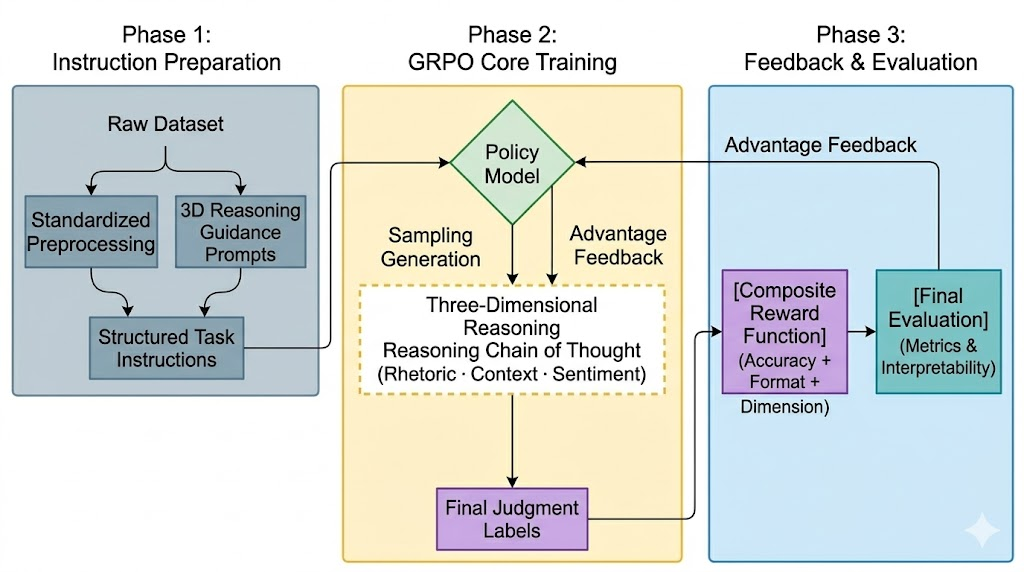
\includegraphics[width=\linewidth]{framework_two.png}
\end{center}
\caption{Framework~2 (RCE+GRPO): three-dimensional reasoning (Rhetoric, Context, Emotion) combined with GRPO reinforcement learning. The reward function encourages dimension coverage alongside classification accuracy.}
\label{fig:fw2}
\end{figure}

\subsection{Framework~3: Hybrid PMP-RCE with GRPO}

Framework~3 is our proposed method that combines PMP pragmatic analysis with RCE structured reasoning in a unified prompt and optimizes the combined behavior with a multi-component GRPO reward.

\paragraph{Three-Phase Hybrid Prompt.}
The hybrid prompt structures reasoning into three phases:

\textit{Phase 1 (Pragmatic Analysis)}: The model performs PMP-style analysis covering implicature, presupposition, speaker intent, polarity, pretense, and meaning gap.

\textit{Phase 2 (Structured Analysis)}: The model performs RCE analysis covering rhetoric, context, and emotion dimensions.

\textit{Phase 3 (Reflection and Calibration)}: The model reassesses both analyses together, identifies evidence for and against sarcasm, and applies calibration rules. A decision rule requires that pragmatic incongruity be supported by at least one structured cue from rhetoric, context, or emotion.

\paragraph{Multi-Component Reward.}
The GRPO reward for Framework~3 combines four components:
\begin{equation}
R = R_{\text{acc}} + 0.15 \cdot R_{\text{fmt}} + 0.20 \cdot R_{\text{pmp}} + 0.20 \cdot R_{\text{rce}}
\end{equation}
where $R_{\text{acc}}$ is the accuracy reward ($+20$ / $-8$), $R_{\text{fmt}}$ rewards valid output format and sufficient reasoning length, $R_{\text{pmp}}$ measures coverage of PMP reasoning dimensions (literal meaning, speaker intent, pragmatic incongruity, affective contrast), and $R_{\text{rce}}$ measures coverage of RCE dimensions (rhetoric, context, emotion) with a bonus for covering all three.

The multi-component design ensures that the model learns to produce correct classifications while maintaining comprehensive reasoning that spans both pragmatic and structural perspectives. Training hyperparameters follow the same configuration as Framework~2. Figure~\ref{fig:fw3} illustrates the hybrid prompt structure and multi-component reward design.

\begin{figure}[htbp]
\begin{center}
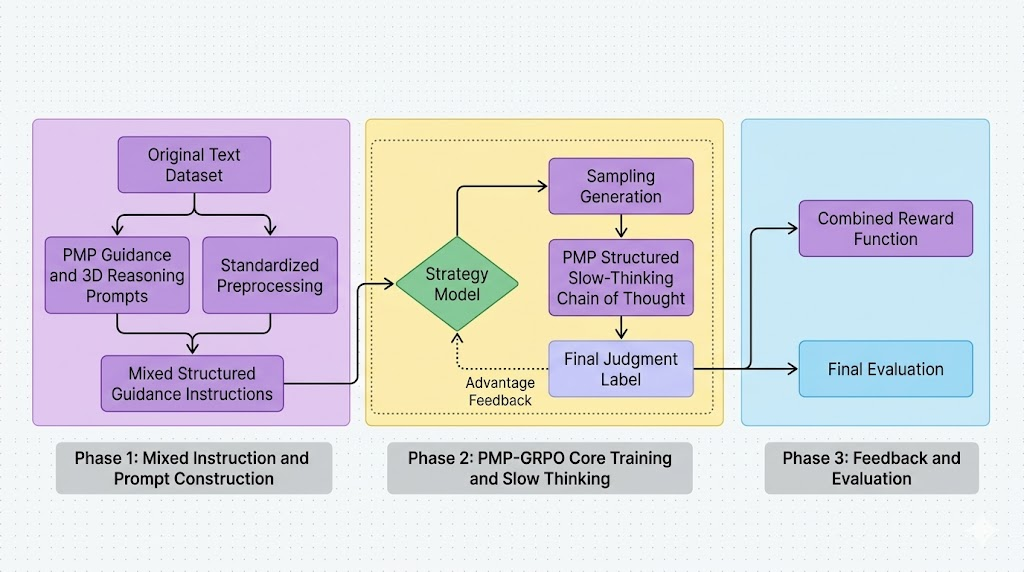
\includegraphics[width=\linewidth]{framework_three.png}
\end{center}
\caption{Framework~3 (Hybrid): three-phase prompt combining PMP pragmatic analysis, RCE structured reasoning, and calibration. The multi-component GRPO reward combines accuracy, format, PMP coverage, and RCE coverage signals.}
\label{fig:fw3}
\end{figure}


\section{Experiments}

\subsection{Datasets}

We evaluate on two test sets derived from SemEval 2018 Task~3~\citep{semeval2018task3}, an English irony detection benchmark:

\begin{itemize}[leftmargin=*, itemsep=0pt]
    \item \textbf{SemEval-200}: A curated subset of 200 samples (80 sarcastic, 120 non-sarcastic), selected to provide a balanced and focused evaluation.
    \item \textbf{SemEval-784}: The full official test set containing 784 samples (311 sarcastic, 473 non-sarcastic).
\end{itemize}

Both datasets use binary labels (sarcastic vs.\ non-sarcastic). Training data for GRPO comes from the SemEval 2018 Task 3 training split.

\subsection{Implementation Details}

All experiments use Qwen3-14B as the base model. Baseline and Framework~1 experiments are inference-only (no parameter updates). Framework~2 and Framework~3 use GRPO training with LoRA (rank 16, alpha 32, dropout 0.05). We use bfloat16 precision with gradient checkpointing. Training runs for 200 steps with batch size 1, gradient accumulation steps 4, and learning rate $3 \times 10^{-6}$ with cosine scheduling. For each prompt, 4 completions are generated and scored by the reward function. Figure~\ref{fig:grpo} illustrates the GRPO training pipeline.

\begin{figure}[htbp]
\begin{center}
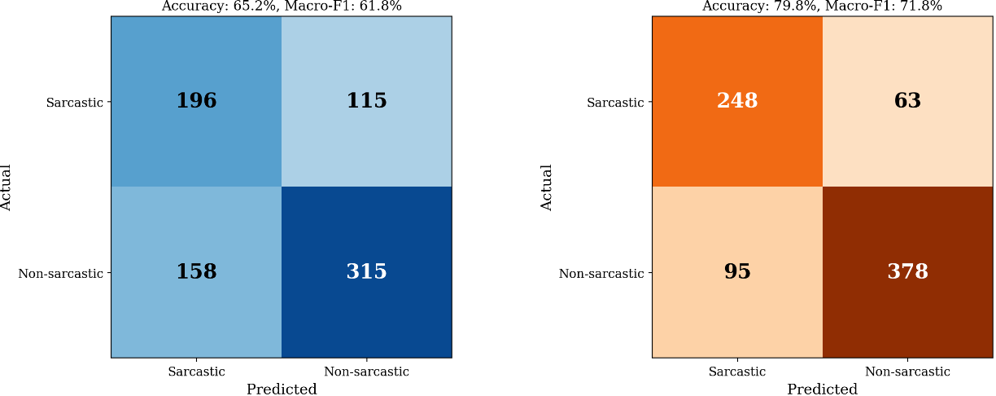
\includegraphics[width=\linewidth]{GRPO.png}
\end{center}
\caption{GRPO training pipeline. For each prompt, multiple completions are generated, scored by the multi-component reward, and used to compute group-relative advantages for policy optimization via LoRA.}
\label{fig:grpo}
\end{figure}

We report Accuracy and Macro-F1 as primary metrics, along with per-class Precision, Recall, and F1 for detailed analysis.

\subsection{Main Results}

\begin{table}[htbp]
\centering
\small
\caption{Main results on SemEval-200 and SemEval-784. Best results in \textbf{bold}.}
\label{tab:main-results}
\resizebox{\textwidth}{!}{%
\begin{tabular}{llcccc}
\toprule
Dataset & Method & Acc. & Macro-F1 & Sarc.\ F1 & Non-Sarc.\ F1 \\
\midrule
\multirow{4}{*}{SemEval-200}
    & Baseline            & 0.610 & 0.595 & 0.672 & 0.519 \\
    & Framework~1 (PMP)   & 0.740 & 0.739 & 0.755 & 0.723 \\
    & Framework~2 (RCE)   & 0.690 & 0.686 & 0.721 & 0.652 \\
    & Framework~3 (Hybrid)& \textbf{0.750} & \textbf{0.750} & \textbf{0.760} & \textbf{0.740} \\
\midrule
\multirow{4}{*}{SemEval-784}
    & Baseline            & 0.579 & 0.560 & 0.652 & 0.468 \\
    & Framework~1 (PMP)   & 0.690 & 0.687 & \textbf{0.718} & 0.655 \\
    & Framework~2 (RCE)   & 0.653 & 0.646 & 0.695 & 0.598 \\
    & Framework~3 (Hybrid)& \textbf{0.695} & \textbf{0.693} & 0.718 & \textbf{0.669} \\
\bottomrule
\end{tabular}
}
\end{table}

Table~\ref{tab:main-results} presents the main results. Figure~\ref{fig:main-results} visualizes the accuracy and Macro-F1 comparison across all methods. Framework~3 achieves the best overall performance on both datasets, with 75.0\% accuracy and 75.0 Macro-F1 on SemEval-200, and 69.5\% accuracy and 69.3 Macro-F1 on SemEval-784.

\begin{figure}[htbp]
\begin{center}
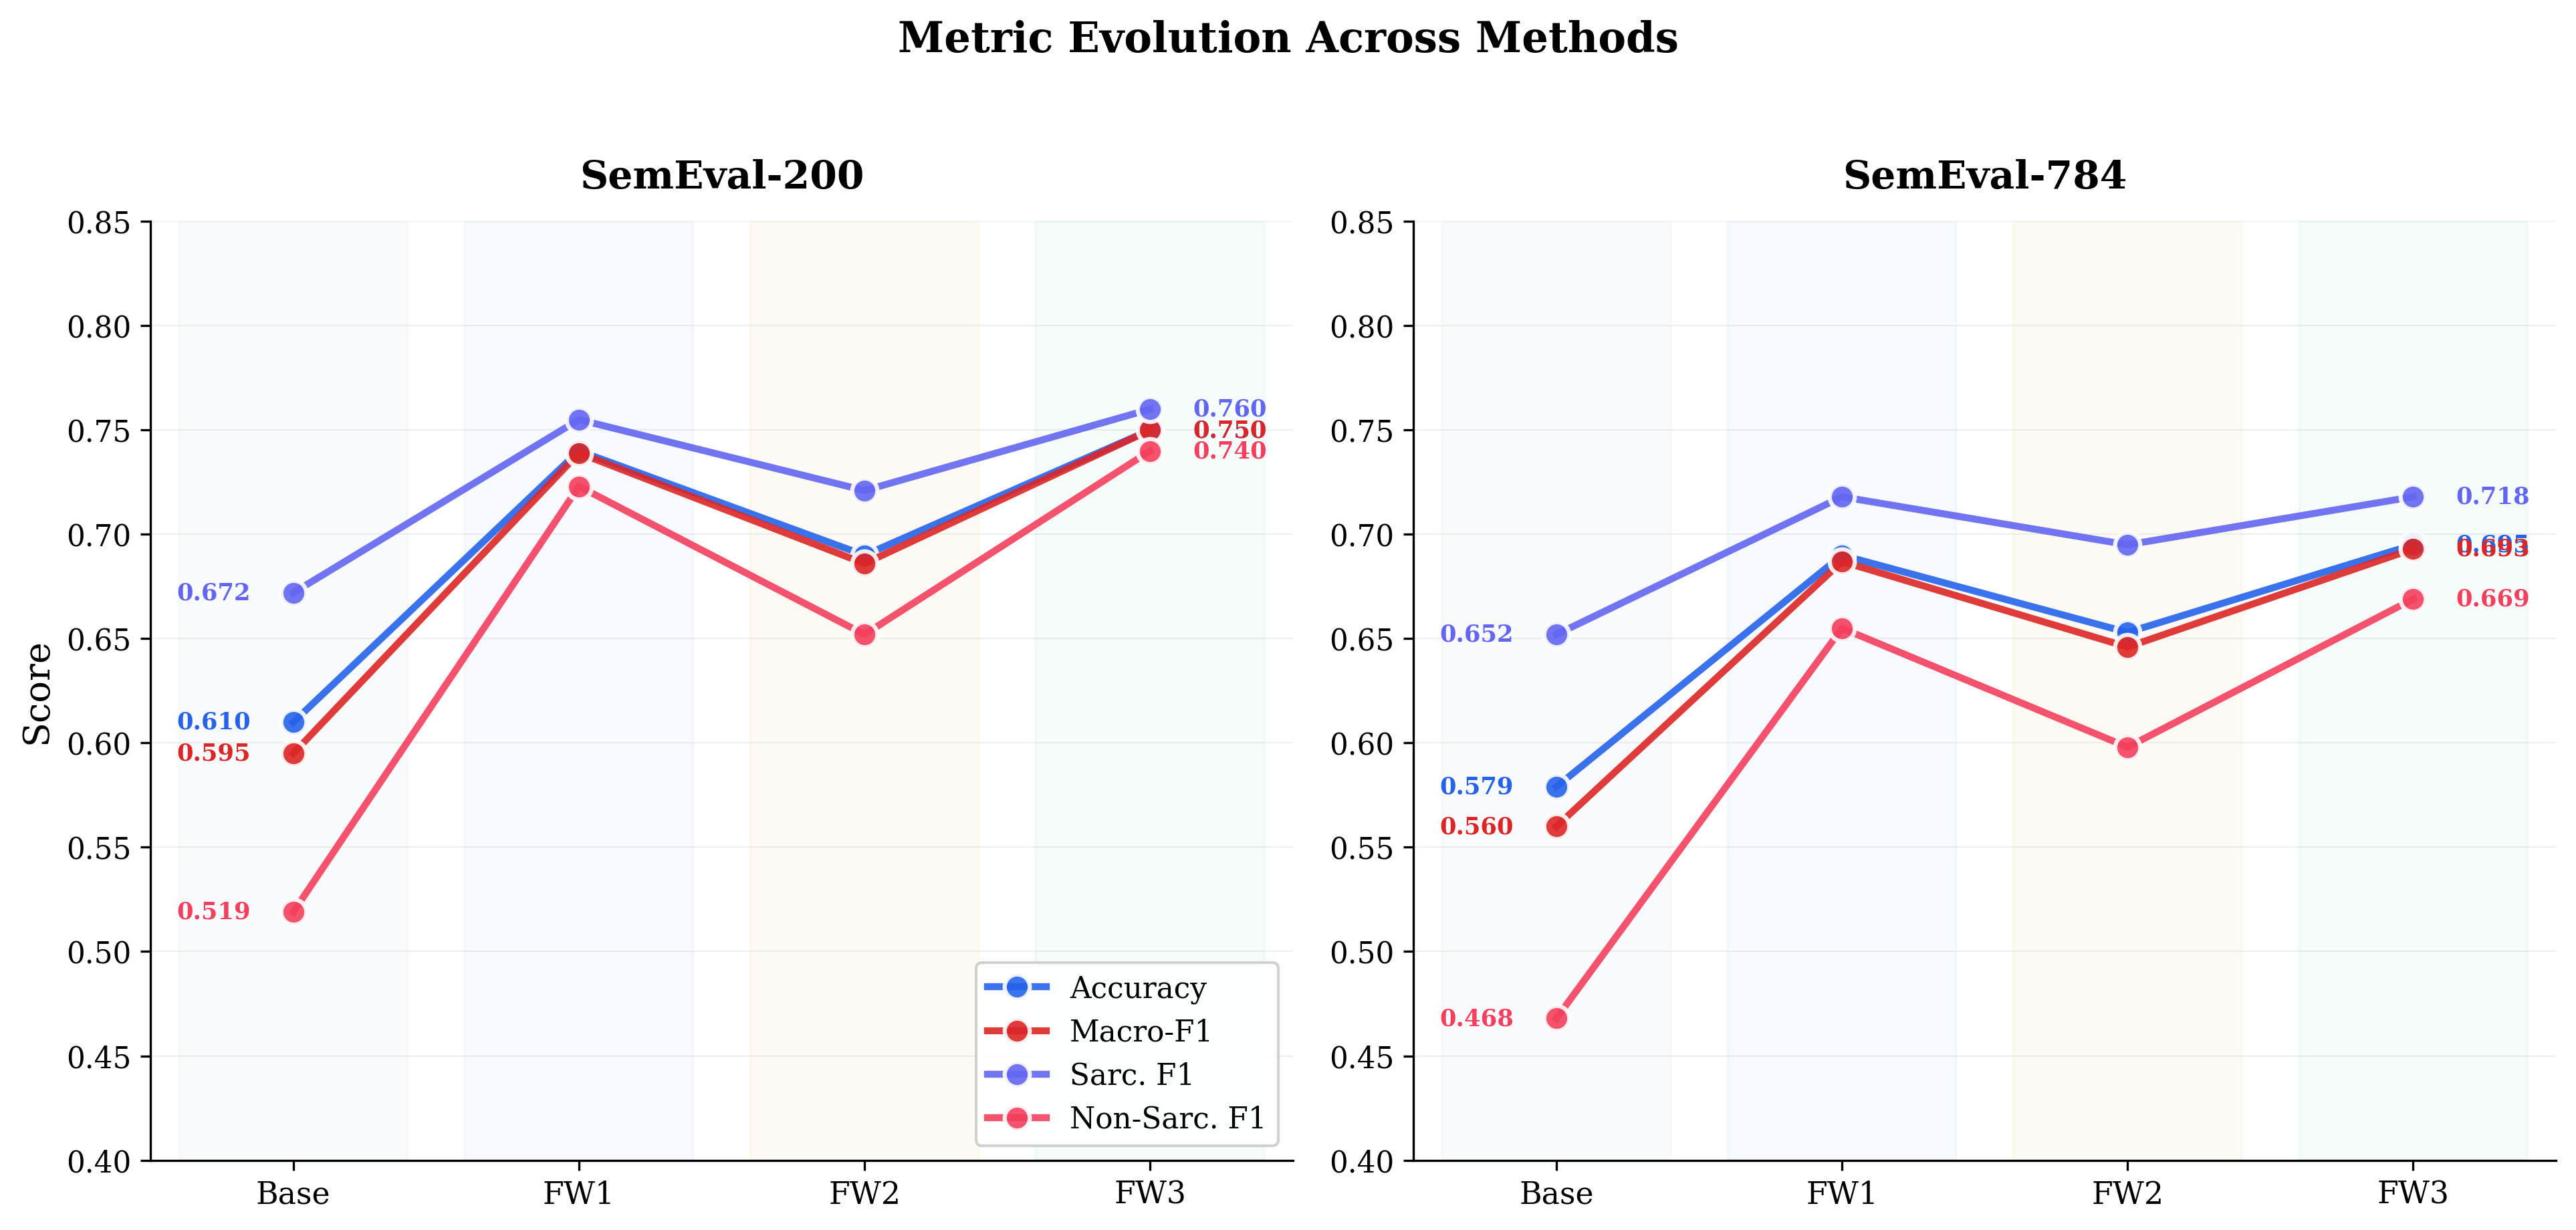
\includegraphics[width=\linewidth]{main_results.png}
\end{center}
\caption{Main results comparison on SemEval-200 and SemEval-784. Framework~3 (Hybrid) consistently achieves the highest accuracy and Macro-F1 on both datasets.}
\label{fig:main-results}
\end{figure}

Several observations emerge from the results:

\paragraph{PMP prompting significantly improves over the baseline.}
Framework~1 achieves substantial gains over the Baseline (+13.0\% accuracy on SemEval-200, +11.1\% on SemEval-784), demonstrating that guiding the model through pragmatic analysis improves sarcasm detection even without any training.

\paragraph{RCE reasoning with GRPO provides consistent improvements.}
Framework~2 outperforms the Baseline by +8.0\% and +7.4\% accuracy on the two datasets, confirming that structured reasoning with GRPO training helps the model produce more informative analyses.

\paragraph{The hybrid approach achieves the best balance.}
Framework~3 improves over Framework~2 by +6.0\% accuracy on SemEval-200 and +4.2\% on SemEval-784. Notably, the largest improvement comes in non-sarcastic F1 (+0.088 on SemEval-200, +0.071 on SemEval-784), indicating that the combined reasoning helps the model better distinguish genuine non-sarcastic text from sarcastic text.

\subsection{Analysis}

\begin{table}[htbp]
\centering
\small
\caption{Confusion matrices on SemEval-784. TP/FP/FN/TN are computed with sarcastic as the positive class.}
\label{tab:confusion}
\begin{tabular}{llrrrr}
\toprule
Dataset & Method & TP & FP & FN & TN \\
\midrule
\multirow{4}{*}{SemEval-784}
    & Baseline            & 309 & 328 &  2 & 145 \\
    & Framework~1 (PMP)   & 310 & 242 &  1 & 231 \\
    & Framework~2 (RCE)   & 310 & 271 &  1 & 202 \\
    & Framework~3 (Hybrid)& 304 & 232 &  7 & 241 \\
\bottomrule
\end{tabular}
\end{table}

\paragraph{False positive reduction.}
A key challenge in sarcasm detection is over-prediction: many models tend to classify negative or emotional text as sarcastic. Table~\ref{tab:confusion} and Figure~\ref{fig:confusion} show that all four methods have high sarcastic recall (TP close to 311), but differ substantially in false positives. The Baseline produces 328 false positives, meaning it labels 69\% of non-sarcastic samples as sarcastic. Framework~1 reduces this to 242, Framework~2 to 271, and Framework~3 further reduces it to 232. Framework~3 achieves the best trade-off: it sacrifices only 7 sarcastic samples (from 310 to 304 TP) while correctly classifying 241 non-sarcastic samples (up from 145 in the baseline).

\begin{figure}[htbp]
\begin{center}
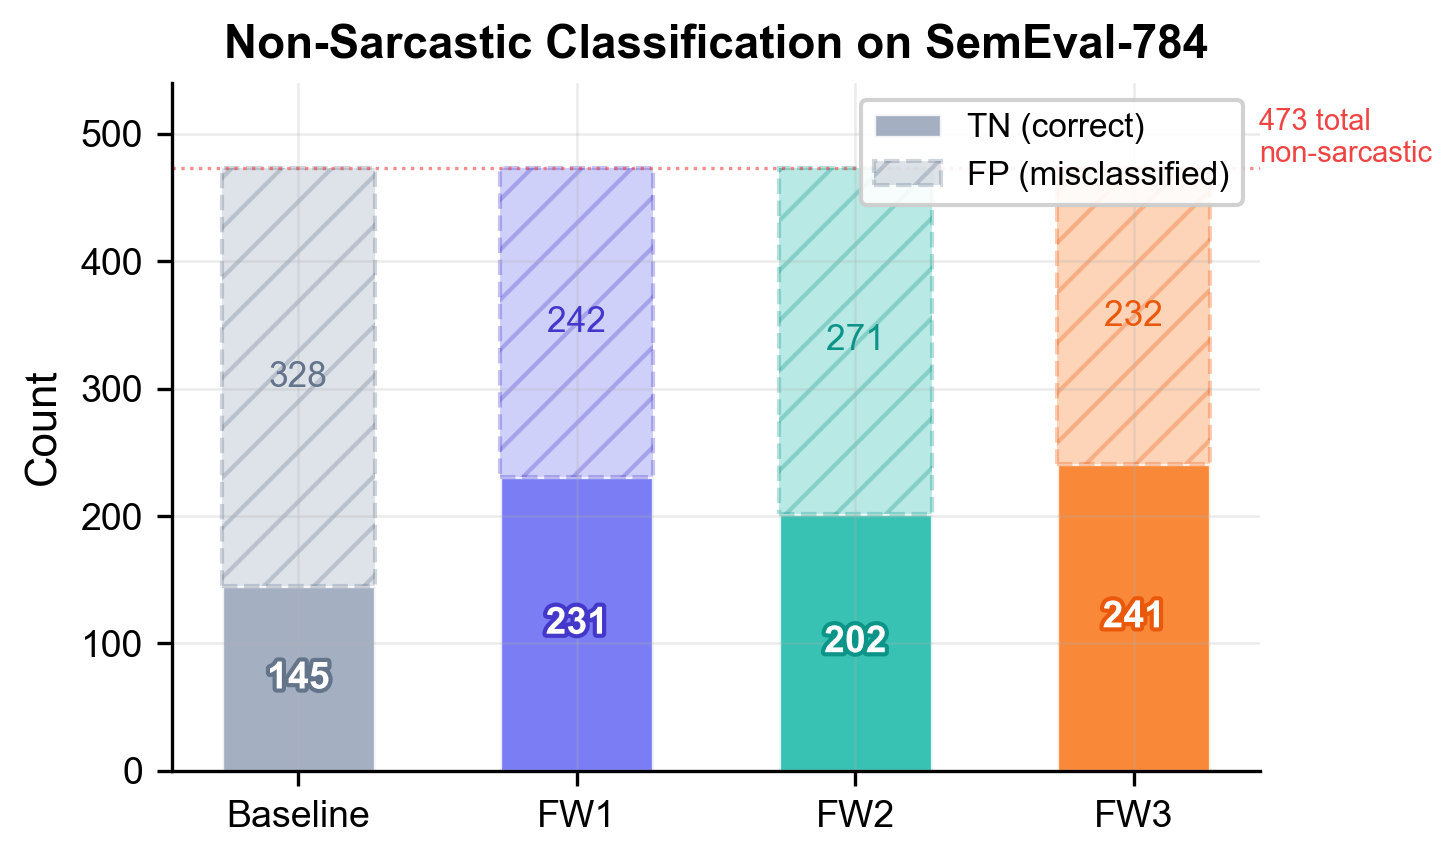
\includegraphics[width=\linewidth]{confusion_flow.png}
\end{center}
\caption{Prediction redistribution on SemEval-784. Solid bars show actual class distribution; dashed bars show predicted distribution. FP counts decrease from Baseline (328) to FW3 (232), reflecting improved non-sarcastic recognition.}
\label{fig:confusion}
\end{figure}

\paragraph{Per-class performance.}
\begin{table}[htbp]
\centering
\small
\caption{Per-class recall on SemEval-784.}
\label{tab:recall}
\begin{tabular}{llcc}
\toprule
Method & Sarc.\ Recall & Non-Sarc.\ Recall & Gap \\
\midrule
Baseline            & 0.994 & 0.307 & 0.687 \\
Framework~1 (PMP)   & 0.997 & 0.488 & 0.509 \\
Framework~2 (RCE)   & 0.997 & 0.427 & 0.570 \\
Framework~3 (Hybrid)& 0.978 & 0.510 & 0.468 \\
\bottomrule
\end{tabular}
\end{table}

Table~\ref{tab:recall} shows per-class recall. All methods achieve near-perfect sarcastic recall but vary widely in non-sarcastic recall. Framework~3 achieves the highest non-sarcastic recall (51.0\%) while maintaining 97.8\% sarcastic recall. The gap between the two recalls is smallest for Framework~3 (0.468), indicating the most balanced classification. Figure~\ref{fig:recall-balance} visualizes this recall gap, and Figure~\ref{fig:per-class-f1} further shows that the F1 gap narrows consistently from Baseline to FW3 on both datasets.

\begin{figure}[htbp]
\begin{center}
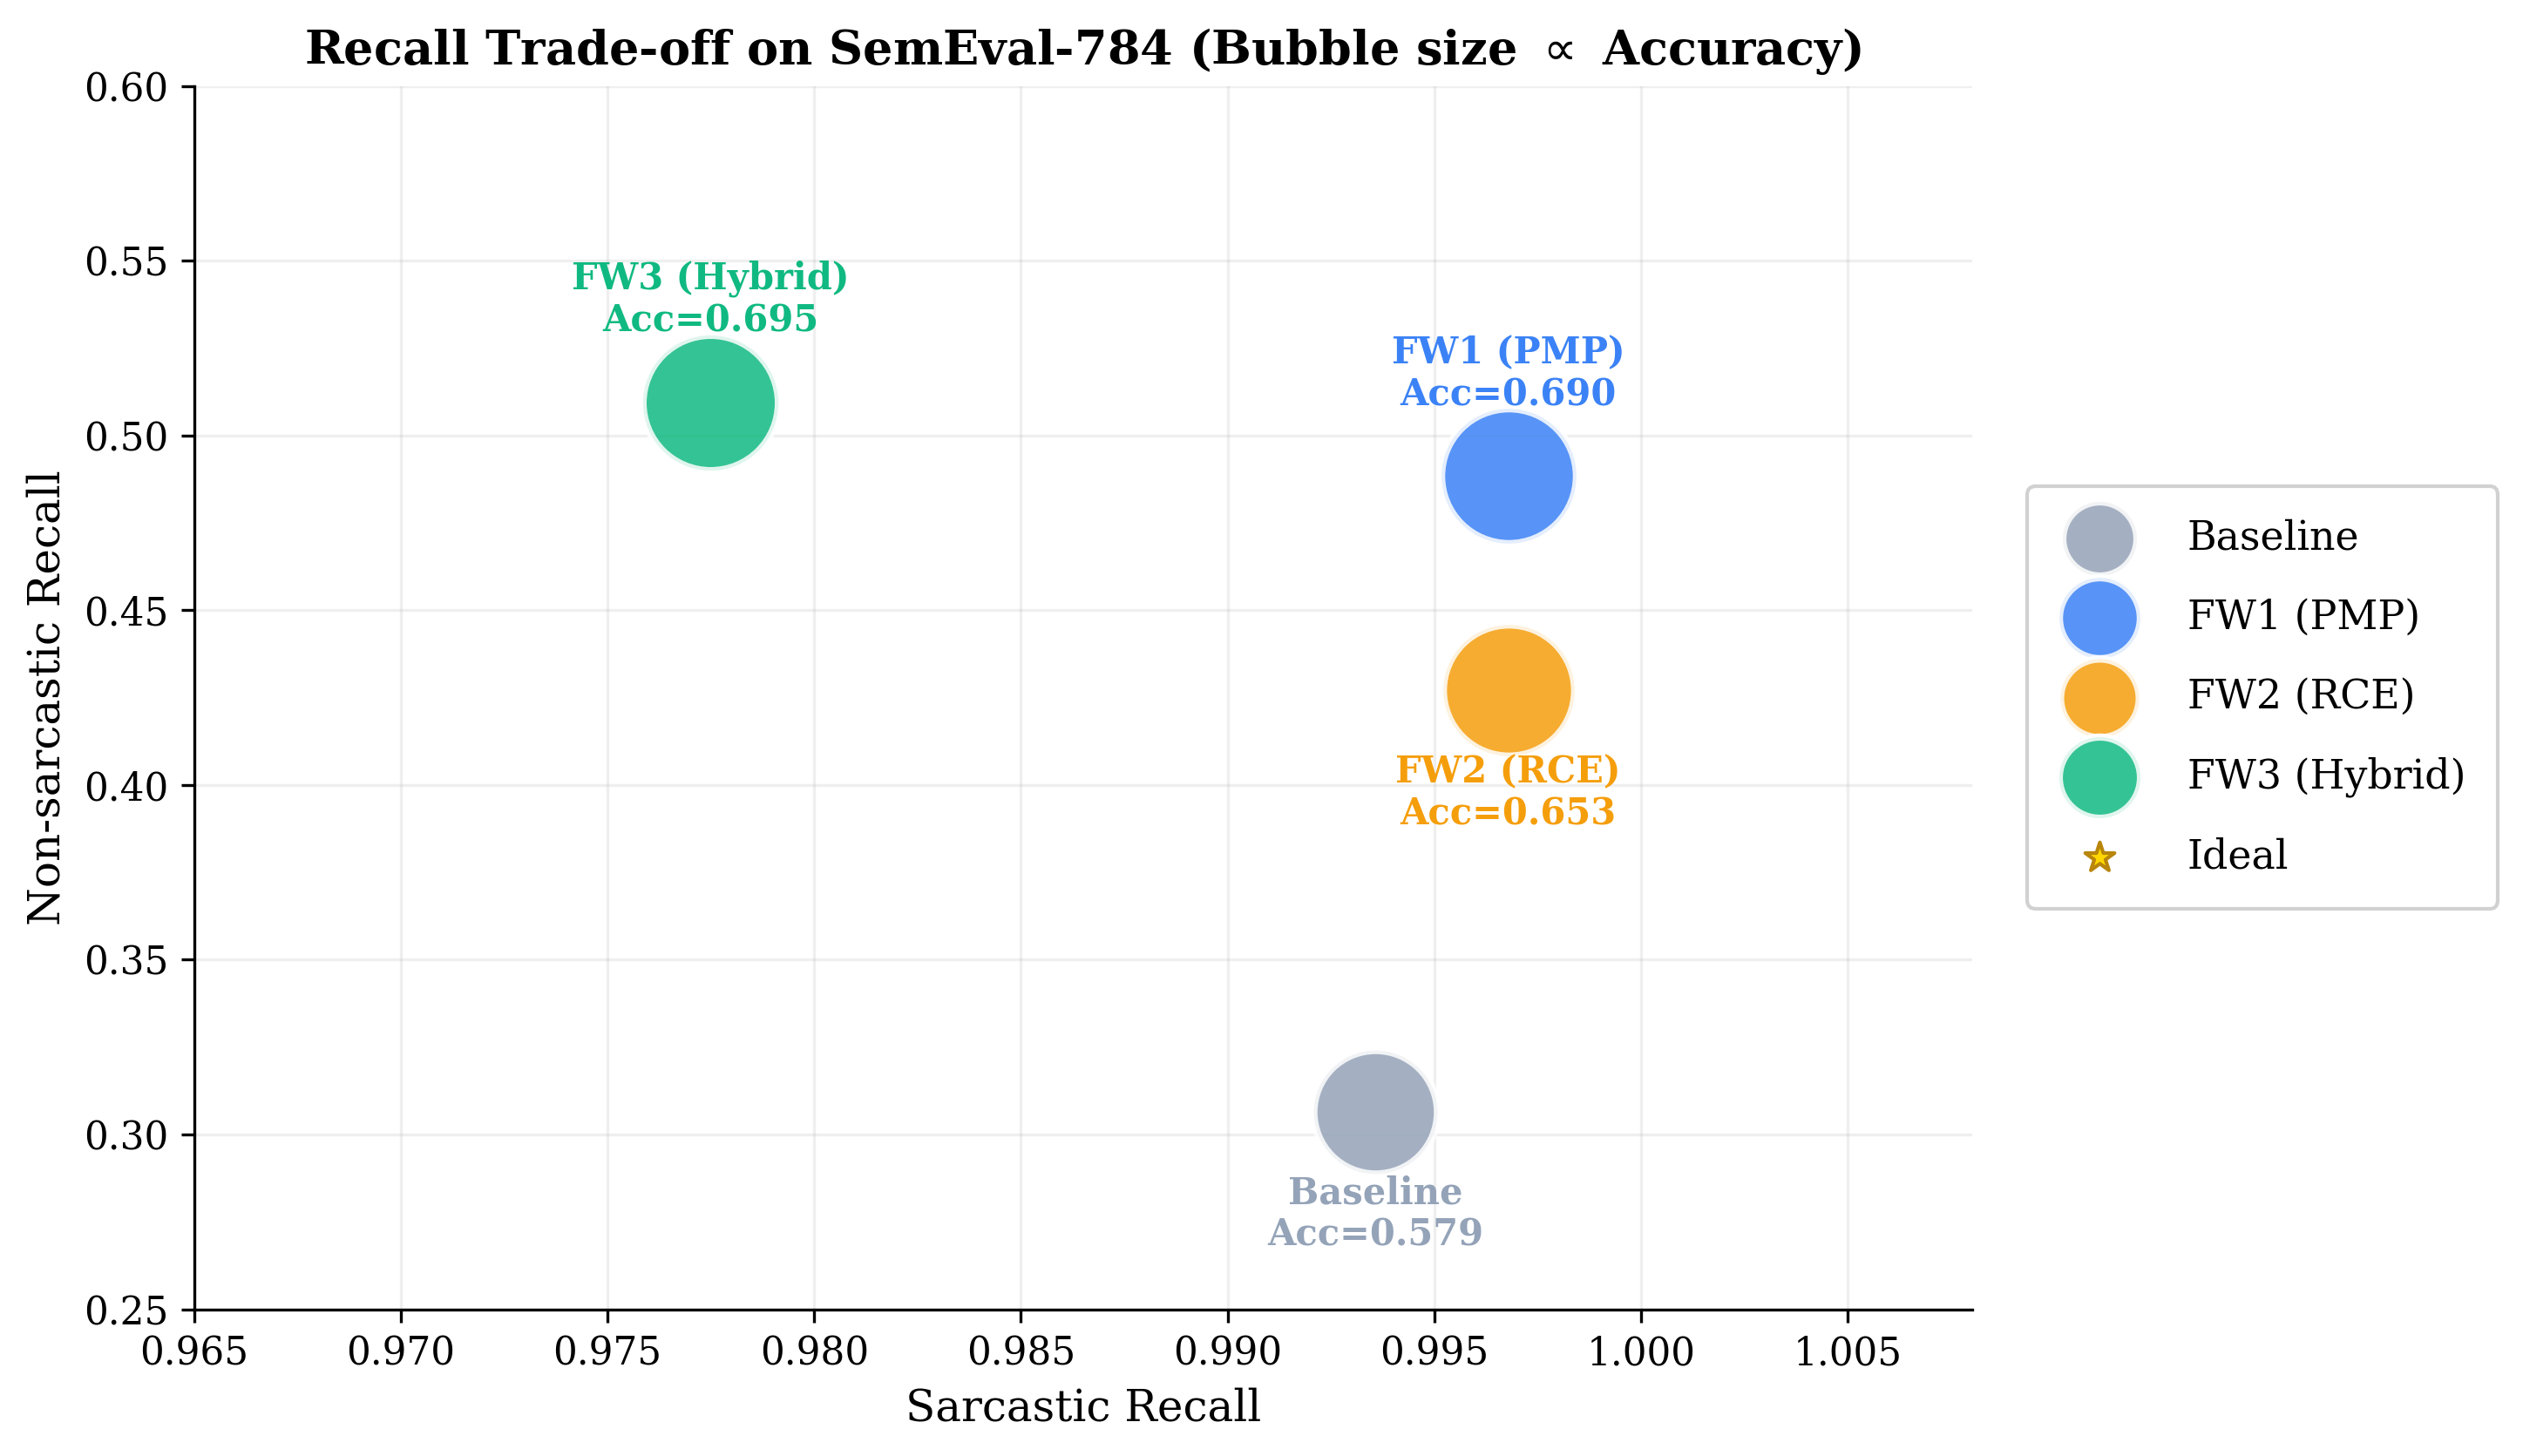
\includegraphics[width=0.85\linewidth]{recall_scatter.png}
\end{center}
\caption{Recall trade-off on SemEval-784. Each bubble represents a method; size is proportional to accuracy. FW3 achieves the best balance with the smallest recall gap (0.468).}
\label{fig:recall-balance}
\end{figure}

\begin{figure}[htbp]
\begin{center}
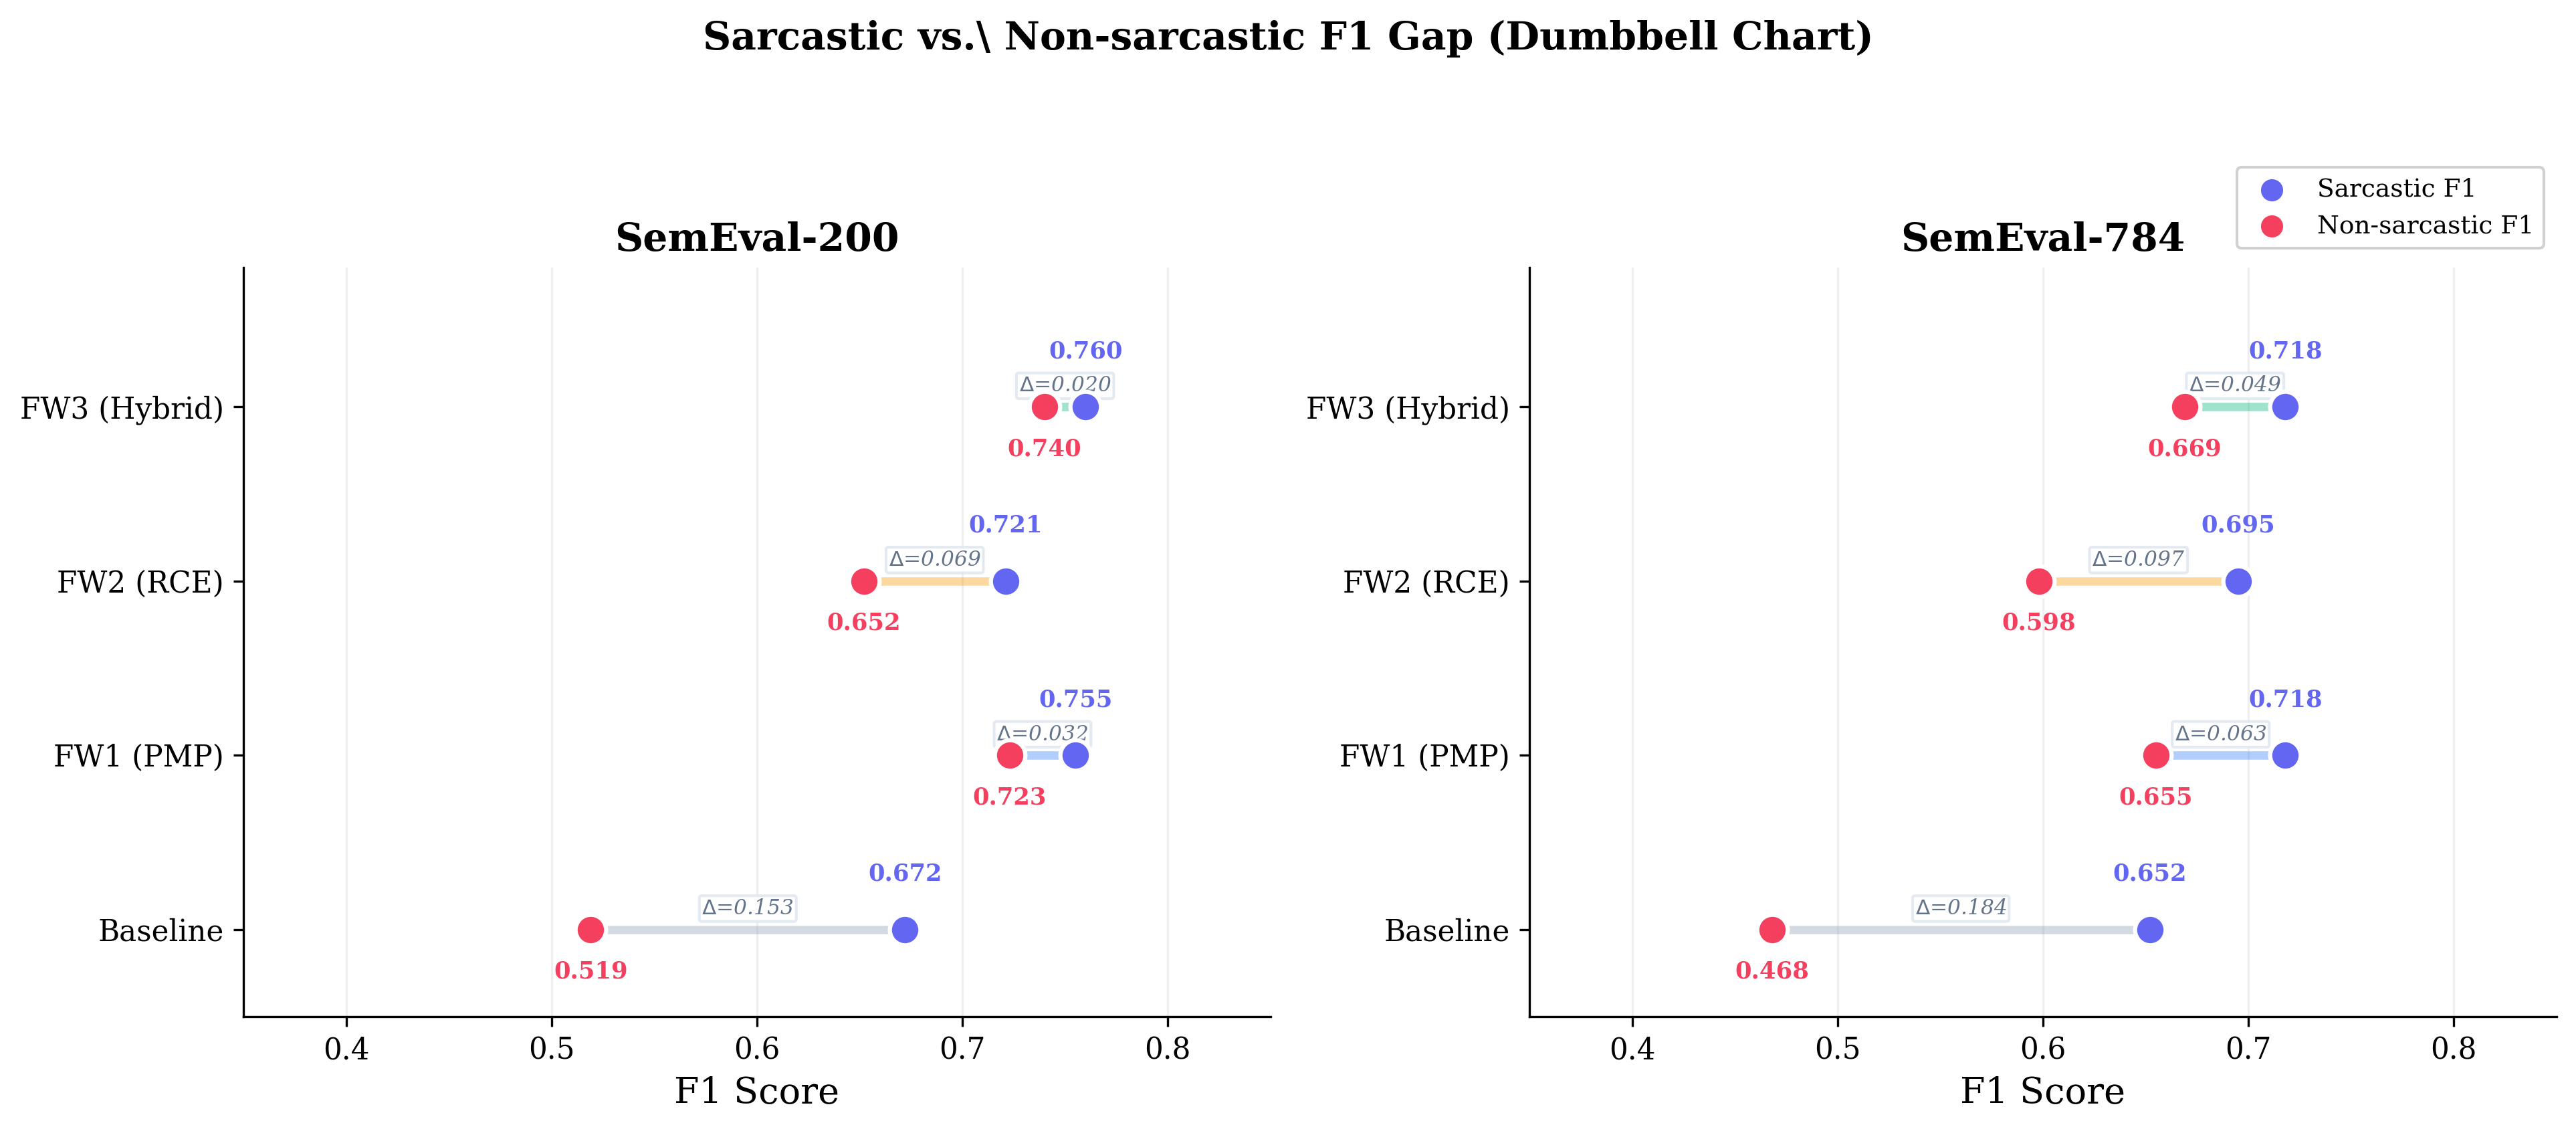
\includegraphics[width=\linewidth]{per_class_f1.png}
\end{center}
\caption{Dumbbell chart showing sarcastic vs.\ non-sarcastic F1 on both datasets. The gap ($\Delta$) narrows from Baseline to FW3, confirming that the hybrid approach achieves better class balance.}
\label{fig:per-class-f1}
\end{figure}

\paragraph{Error correction analysis.}
We conduct a pairwise error analysis between frameworks. On SemEval-784, Framework~3 corrects 54 samples that Framework~2 misclassifies while introducing only 21 new errors, yielding a net gain of +33 correct predictions (Figure~\ref{fig:error-corr}). Compared to Framework~1, Framework~3 corrects 148 errors while introducing only 7, a net gain of +141. This demonstrates that the improvement is stable and not due to random variation.

\begin{figure}[htbp]
\begin{center}
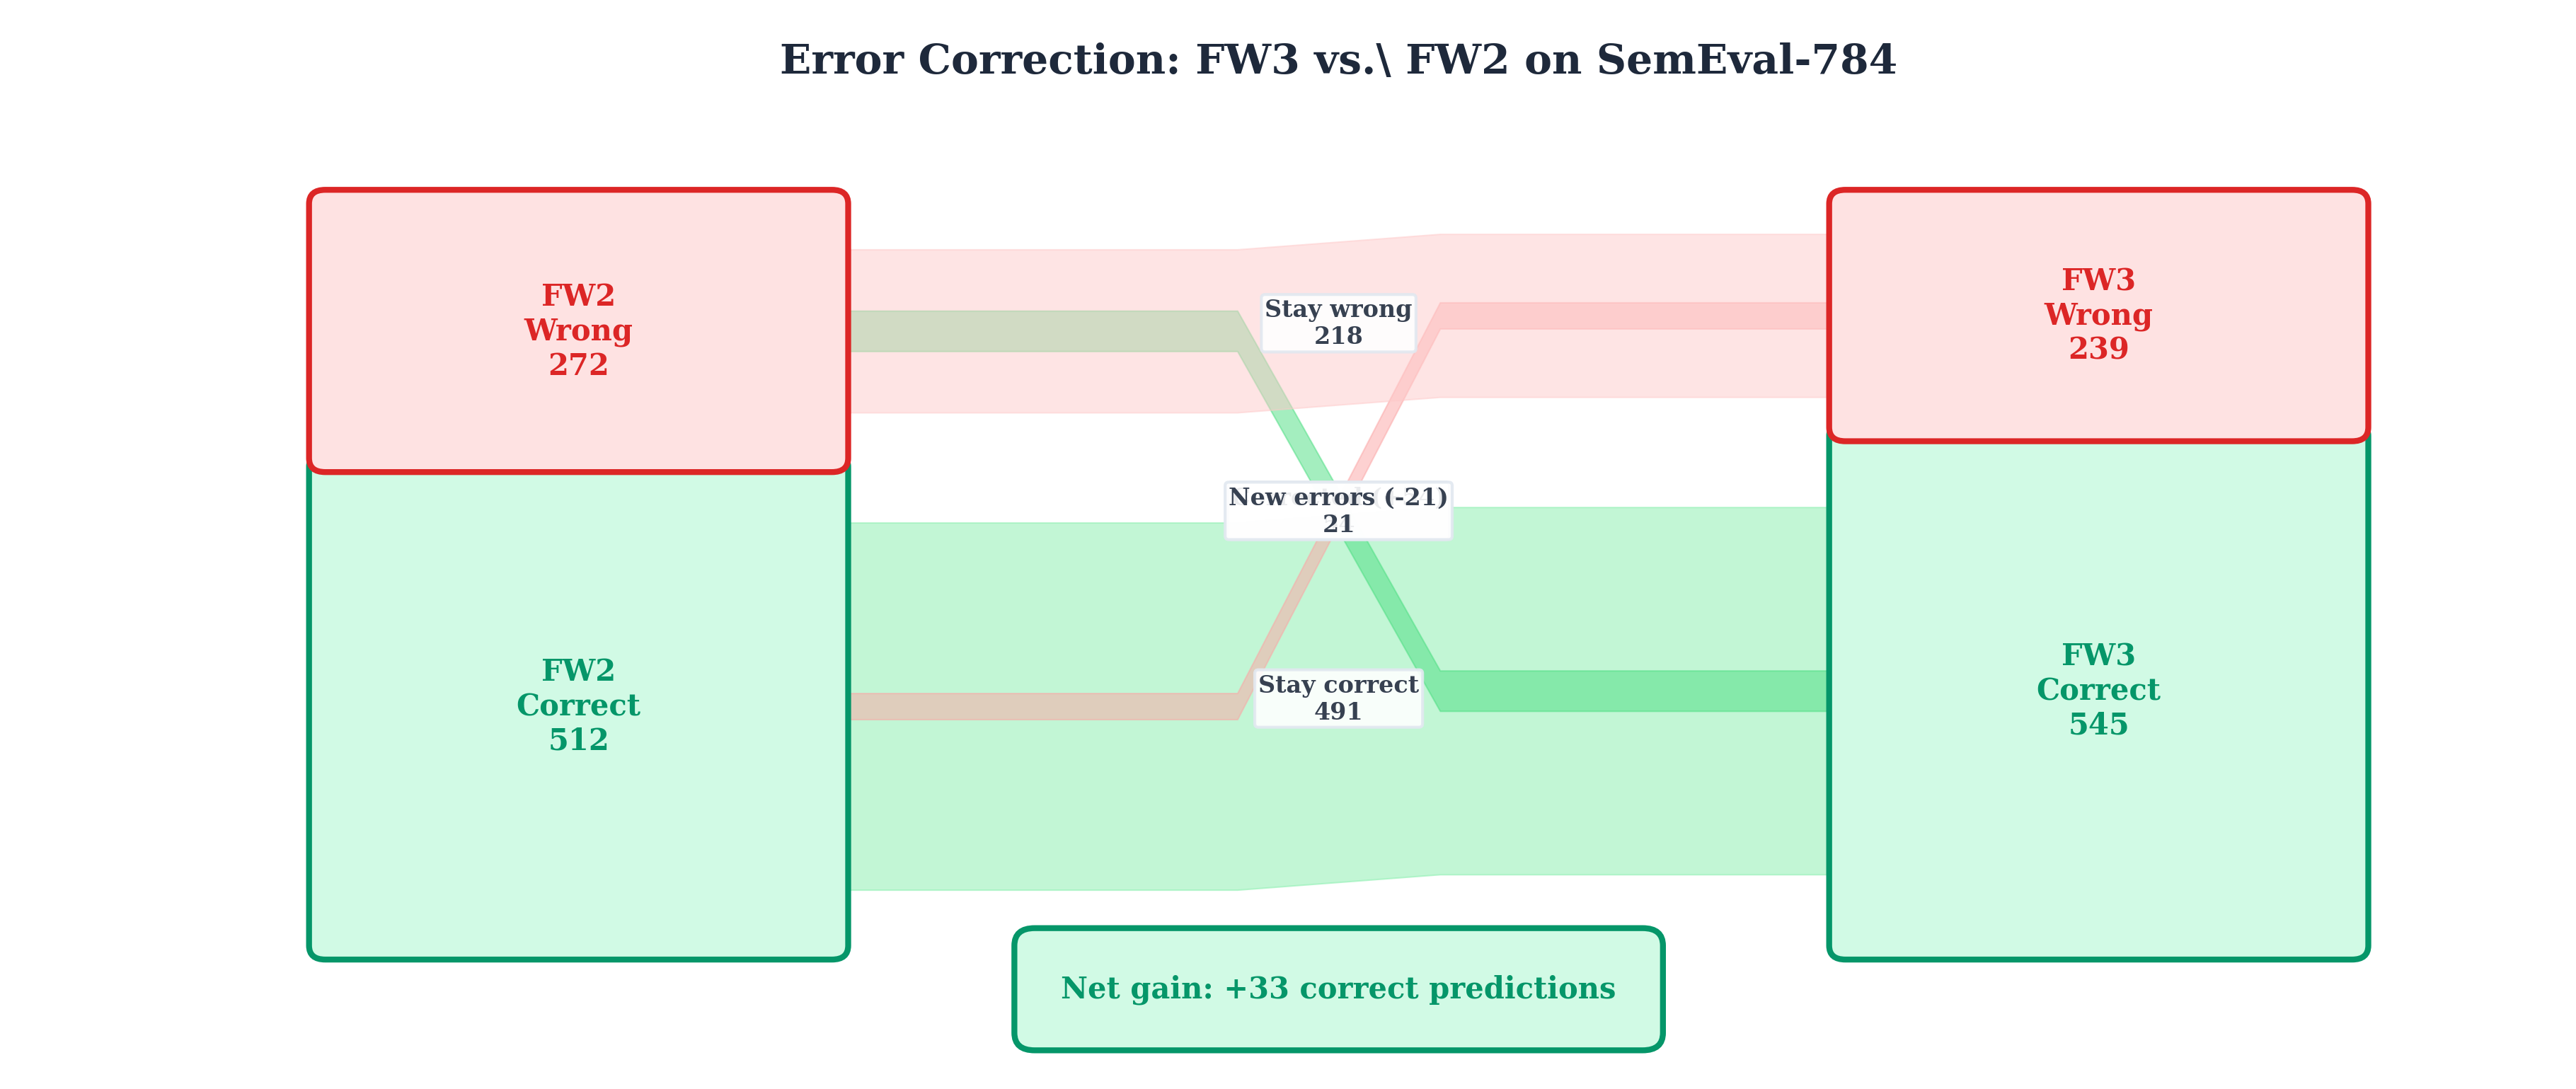
\includegraphics[width=\linewidth]{error_correction.png}
\end{center}
\caption{Error correction flow: FW3 vs.\ FW2 on SemEval-784. FW3 corrects 54 of FW2's errors while introducing only 21 new errors, yielding a net gain of +33 correct predictions.}
\label{fig:error-corr}
\end{figure}

\paragraph{Effectiveness of hybrid reasoning.}
The hybrid prompt ensures that the model considers both pragmatic incongruity and structured linguistic cues before making a decision. The PMP phase catches cases where the literal meaning contradicts the implied meaning, while the RCE phase provides concrete evidence from rhetorical devices, contextual mismatch, or emotional reversal. The calibration phase prevents the model from relying on a single type of evidence, requiring agreement between pragmatic and structural signals. This dual-verification mechanism is the main driver behind the reduced false positive rate. Figure~\ref{fig:heatmap} provides a comprehensive metric heatmap confirming FW3's superiority across all metrics, and Figure~\ref{fig:radar} shows the full radar profile of each method.

\begin{figure}[htbp]
\begin{center}
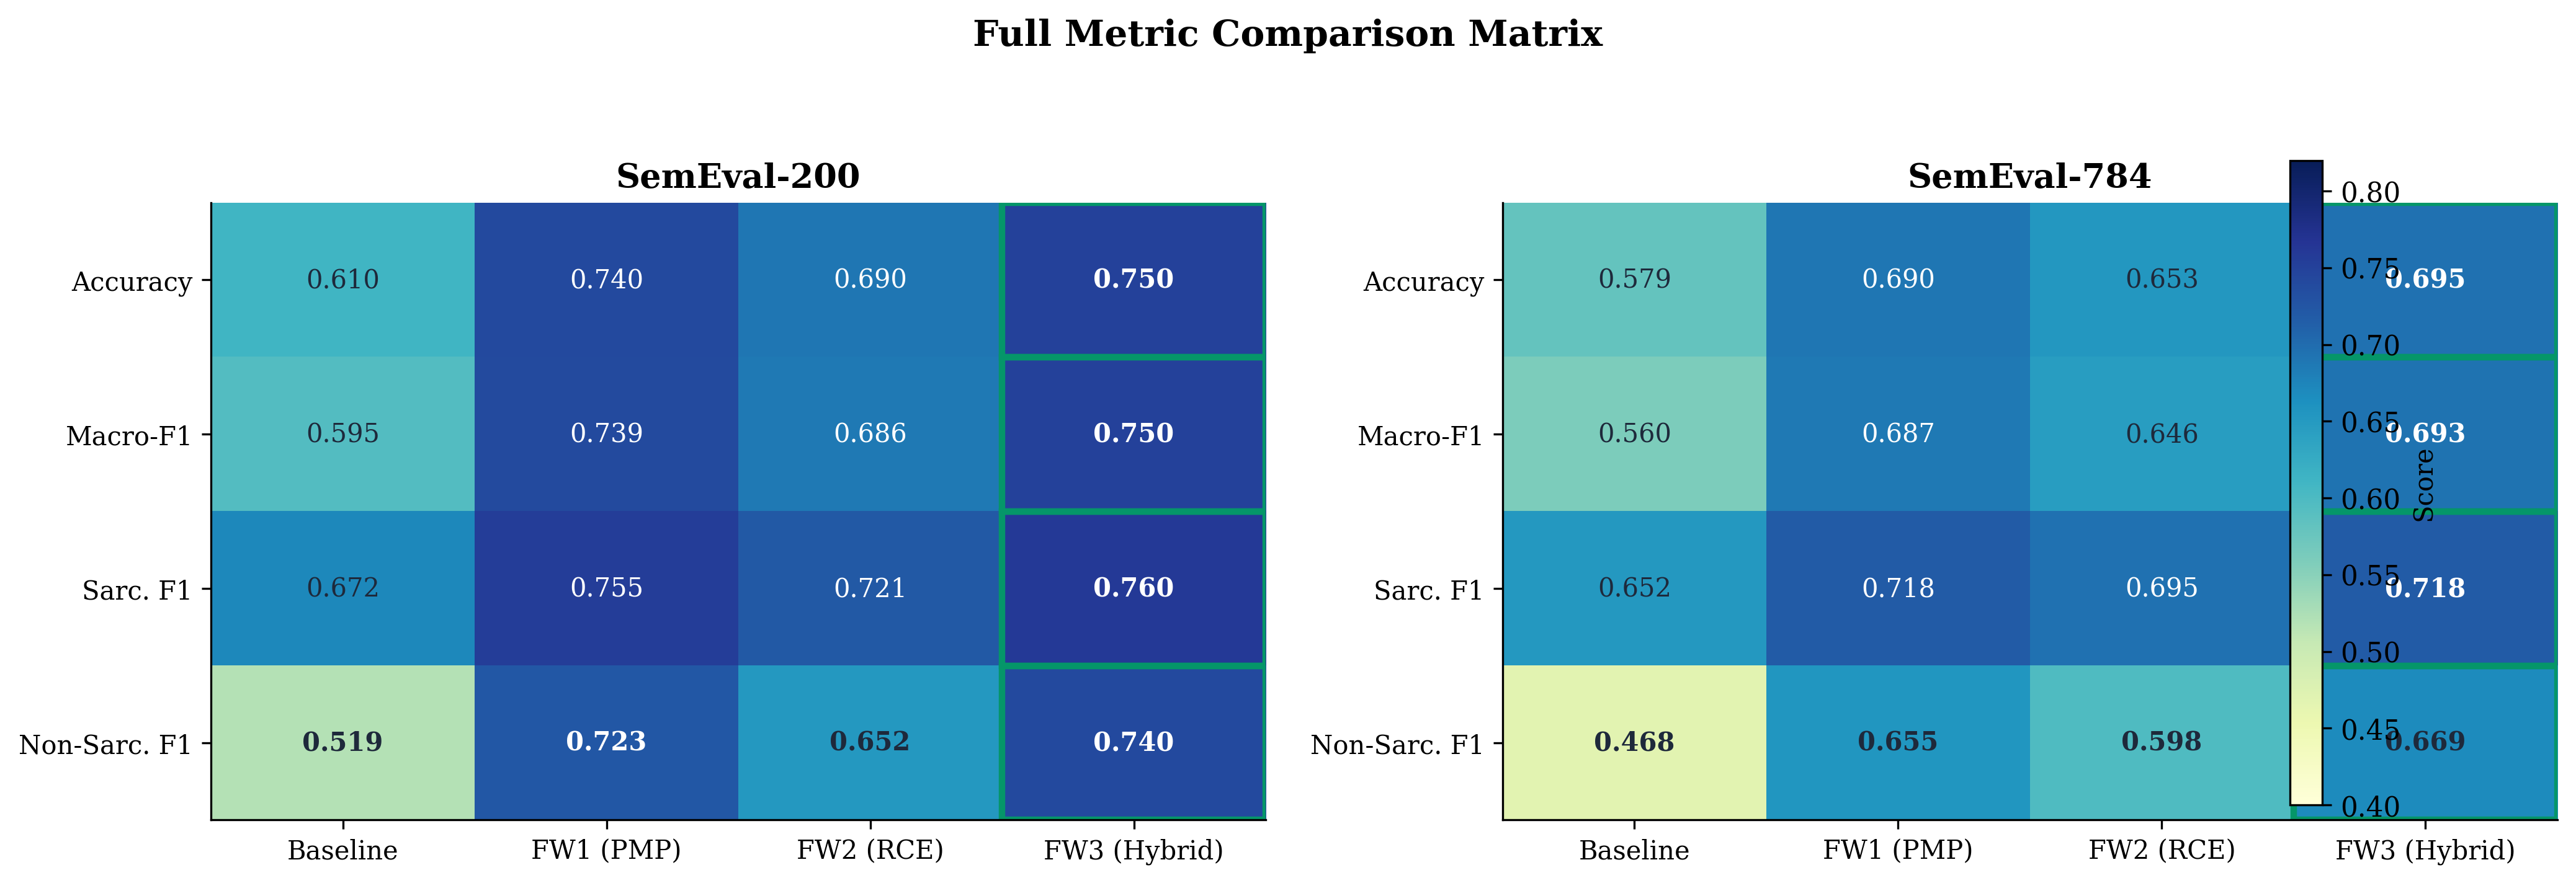
\includegraphics[width=\linewidth]{metric_heatmap.png}
\end{center}
\caption{Metric heatmap for all methods on both datasets. The orange border highlights FW3 as the best-performing method. Darker cells indicate higher scores.}
\label{fig:heatmap}
\end{figure}

\begin{figure}[htbp]
\begin{center}
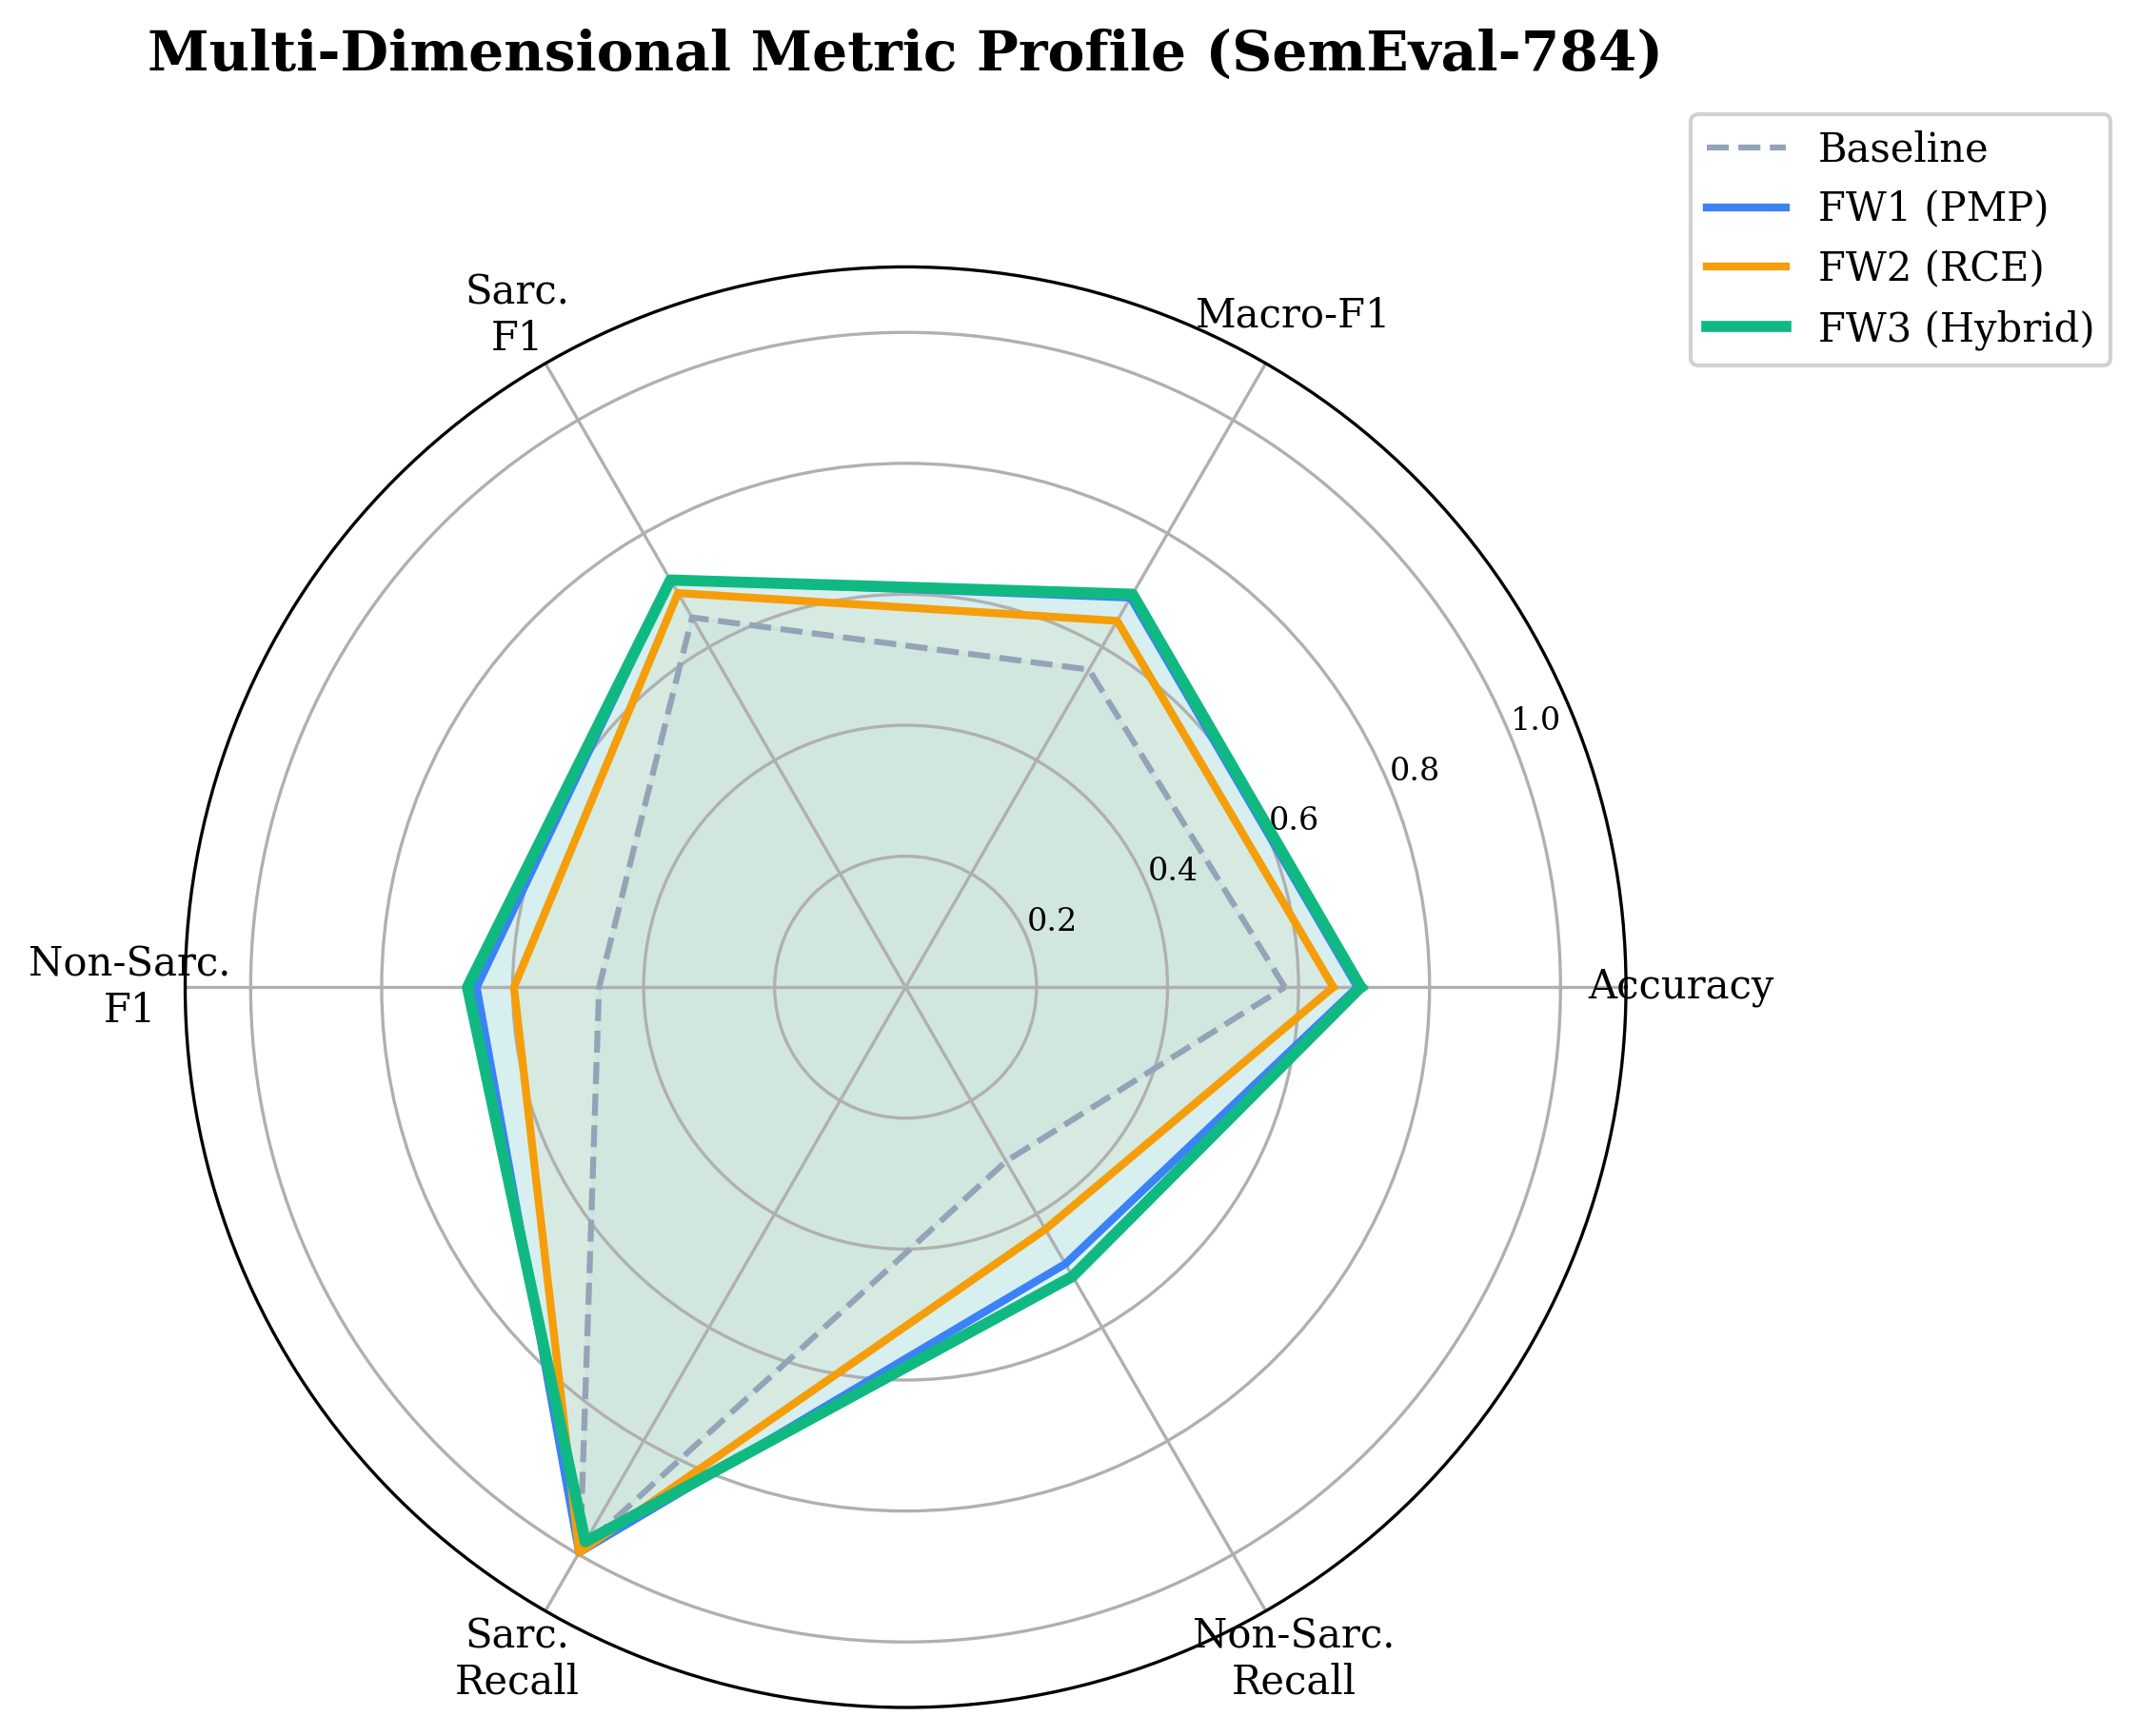
\includegraphics[width=0.7\linewidth]{radar_metrics.png}
\end{center}
\caption{Radar chart of metric profiles on SemEval-784. FW3 shows the most balanced profile with the highest scores across most dimensions. All methods exhibit high sarcastic recall but vary in non-sarcastic recall.}
\label{fig:radar}
\end{figure}

\subsection{Prompt Strategy and Model Scaling Analysis}

To understand when and why PMP helps, we conduct an additional analysis comparing nine prompt strategies on Qwen3-14B, and measure how each strategy changes when scaling from Qwen2-7B to Qwen3-14B.

\begin{table}[htbp]
\centering
\small
\caption{Nine prompt strategies on Qwen3-14B (SemEval-200). Values are percentages.}
\label{tab:prompt-comp}
\begin{tabular}{lrrrr}
\toprule
Method & Acc. & Macro-F1 & Sarc.\ F1 & Correct \\
\midrule
CoT & 78.0 & 78.0 & 77.8 & 156/200 \\
Full PMP & 78.0 & 78.0 & 77.3 & 156/200 \\
CoC & 77.5 & 77.5 & 78.1 & 155/200 \\
PMP two-call & 73.0 & 73.0 & 72.5 & 146/200 \\
ToT & 73.0 & 73.0 & 72.2 & 146/200 \\
IO & 72.0 & 71.9 & 73.3 & 144/200 \\
BoC & 71.0 & 70.8 & 73.4 & 142/200 \\
Baseline & 57.5 & 55.4 & 65.0 & 115/200 \\
GoC & 54.0 & 50.7 & 63.5 & 108/200 \\
\bottomrule
\end{tabular}
\end{table}

Table~\ref{tab:prompt-comp} shows that Full PMP and CoT are tied at 78.0\% accuracy, with CoC close behind at 77.5\%. This demonstrates that PMP's pragmatic decomposition is competitive with general chain-of-thought reasoning when the model has sufficient capacity. However, PMP is not uniquely dominant---CoT reaches the same accuracy, suggesting that structured reasoning (whether pragmatic or general) is the key factor.

\paragraph{Model scaling effect.}
Figure~\ref{fig:delta} visualizes the Macro-F1 change when scaling from Qwen2-7B to Qwen3-14B. The pattern reveals a clear split: reasoning-heavy prompts (Full PMP: +16.1, PMP two-call: +15.7, CoT: +17.7, ToT: +15.0) benefit substantially from larger models, while direct or poorly calibrated prompts degrade (Baseline: $-$17.5, GoC: $-$22.7, IO: $-$6.6). This indicates that model scaling does not uniformly improve all prompt formats. Larger models better exploit structured reasoning instructions but can also become more sensitive to underspecified prompts.

\begin{figure}[htbp]
\centering
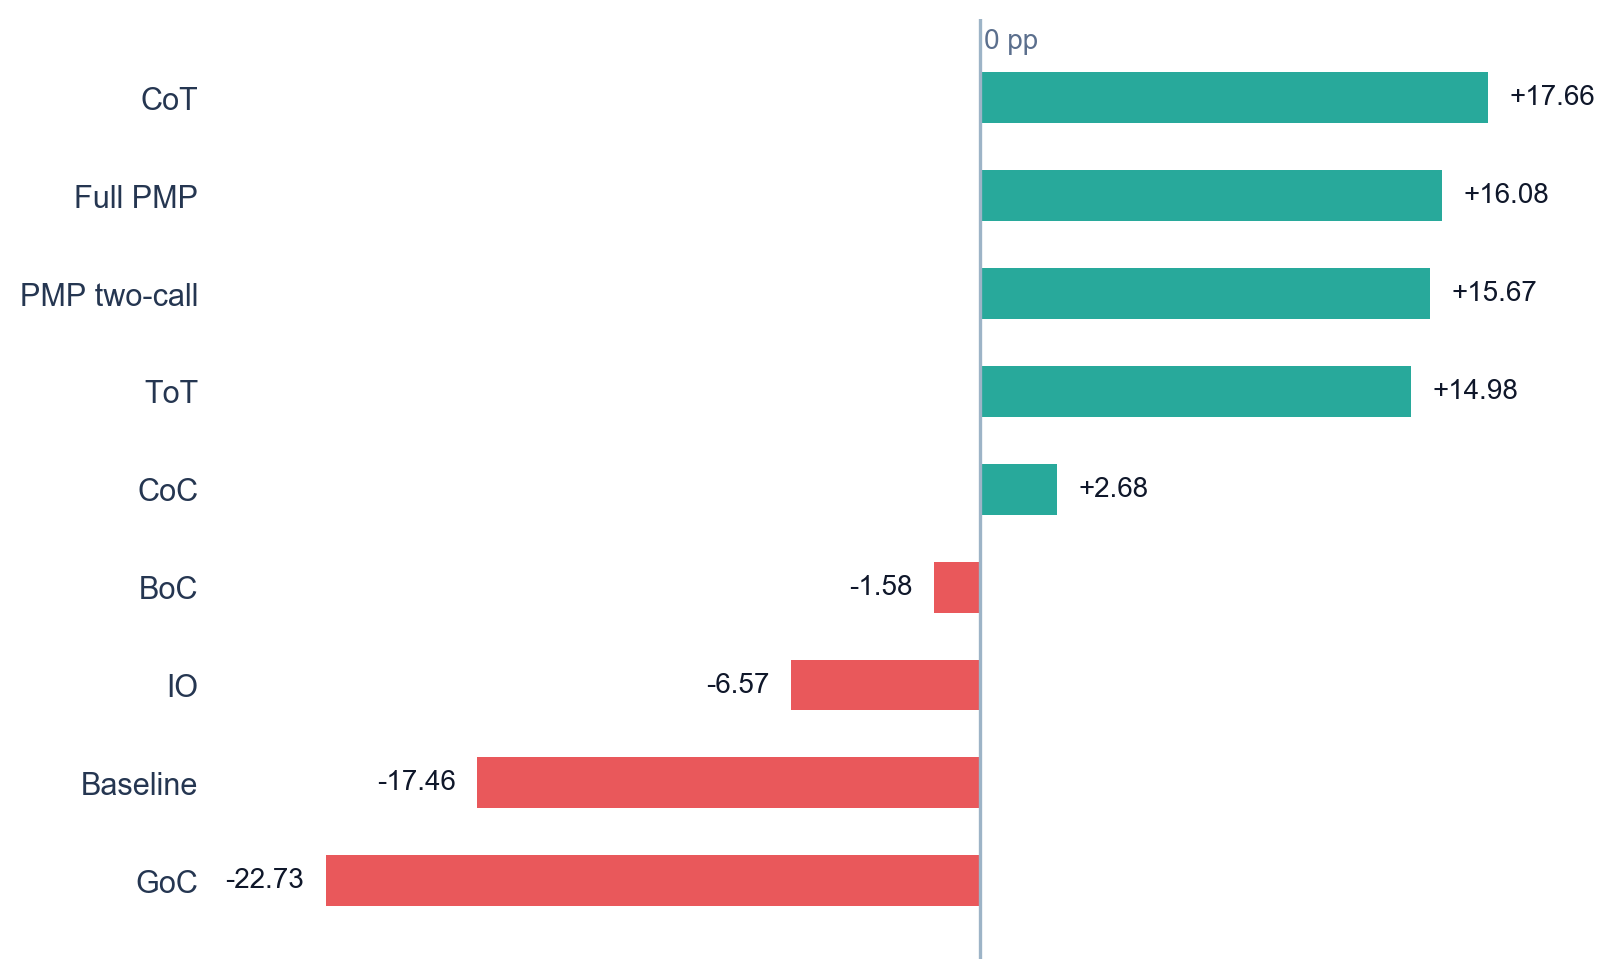
\includegraphics[width=0.86\linewidth]{prompt_delta_stat_only.png}
\caption{Macro-F1 change from Qwen2-7B to Qwen3-14B for each prompt strategy. Reasoning-heavy prompts benefit from model scaling; direct prompts can degrade.}
\label{fig:delta}
\end{figure}

\paragraph{Full PMP vs.\ PMP two-call.}
Full PMP (78.0\%) outperforms PMP two-call (73.0\%) on Qwen3-14B. Although the two-call design separates analysis and reflection, the second call can introduce inconsistency: the model may reinterpret its previous response in a way that changes the final label without improving evidence quality. Full PMP avoids this by keeping analysis, reflection, and decision in one generation, reducing cross-turn drift.


\section{Conclusion}

We presented a systematic study of four approaches to sarcasm detection using the same base LLM. Our results demonstrate that combining pragmatic metacognitive analysis with structured rhetoric-context-emotion reasoning, optimized through GRPO with multi-component rewards, leads to the best overall performance. The hybrid framework achieves 75.0\% accuracy on SemEval-200 and 69.5\% on SemEval-784, with the most balanced per-class performance. The key insight is that sarcasm detection benefits from requiring agreement between multiple reasoning perspectives: pragmatic incongruity alone or linguistic cues alone are insufficient, but their combination provides a more reliable signal.

Future work could explore extending the hybrid approach to multimodal sarcasm detection, incorporating visual and audio cues alongside textual reasoning.


\section*{Author Contributions}
W.L.\ implemented the RCE reasoning framework and GRPO training pipeline (Framework~2). X.Z.\ developed the PMP prompting approach (Framework~1) and conducted baseline experiments. Z.Y.\ designed the hybrid framework (Framework~3), implemented the multi-component reward function, and ran the full evaluation pipeline.

\section*{Acknowledgments}
We thank the organizers of SemEval 2018 Task~3 for providing the benchmark dataset.

\section*{Ethics Statement}
This work uses publicly available datasets for sarcasm detection research. All data was collected from public social media posts as part of the SemEval shared task. No personal or sensitive information is used. The models are intended for research purposes in sentiment analysis and should not be deployed for surveillance or monitoring of individuals.


\newpage
\bibliography{colm2026_conference}
\bibliographystyle{colm2026_conference}

\newpage
\appendix
\section{Appendix}

\subsection{PMP Two-Phase Inference (Framework~1)}

Algorithm~\ref{alg:pmp} describes the Pragmatic Metacognitive Prompting inference used in Framework~1. No parameter training is involved; the model is prompted with a two-phase template and produces both reasoning and a final label in a single generation.

\begin{algorithm}[htbp]
\caption{PMP Two-Phase Inference (Framework~1)}
\label{alg:pmp}
\begin{algorithmic}[1]
\REQUIRE Input text $x$, LLM $M$
\STATE $P_1 \leftarrow$ \textsc{Phase1Prompt}: ``Analyze six pragmatic dimensions:''
\STATE \quad $d_1$: \textit{implicature} --- what is implied beyond literal wording
\STATE \quad $d_2$: \textit{presupposition} --- background assumptions the text relies on
\STATE \quad $d_3$: \textit{speaker intent} --- what the speaker appears to achieve
\STATE \quad $d_4$: \textit{polarity} --- surface tone (positive / negative / neutral)
\STATE \quad $d_5$: \textit{pretense} --- speaker pretending an attitude they do not hold?
\STATE \quad $d_6$: \textit{meaning gap} --- clear difference between literal and implied?
\STATE $P_2 \leftarrow$ \textsc{Phase2Prompt}: ``Reflect and calibrate:''
\STATE \quad Identify evidence \textbf{for} sarcasm and \textbf{against} sarcasm
\STATE \quad Do not label sarcastic just because text is negative or emotional
\STATE \quad Require clear pragmatic incongruity for \texttt{sarcastic}
\STATE $P \leftarrow \text{``Text: ''} + x + P_1 + P_2 + \text{``Output: Reflection + [Final] \{label\}''}$
\STATE $o \leftarrow M(P)$ \COMMENT{Single model generation}
\STATE Extract reflection sentence and final label $\hat{y}$ from $o$
\RETURN $\hat{y} \in \{\texttt{sarcastic}, \texttt{non\_sarcastic}\}$, reflection text
\end{algorithmic}
\end{algorithm}

\subsection{Answer Extraction}

Algorithm~\ref{alg:extract} shows the answer extraction procedure shared by all frameworks. It parses the model's free-form output using cascading pattern matching to recover the sarcasm label.

\begin{algorithm}[htbp]
\caption{Answer Extraction from Model Output}
\label{alg:extract}
\begin{algorithmic}[1]
\REQUIRE Model output text $o$
\STATE \textbf{Step 1}: Search for \texttt{[Final] \{sarcastic\}} or \texttt{[Final] \{non\_sarcastic\}}
\IF{matched}
    \RETURN normalized label $\hat{y}$
\ENDIF
\STATE \textbf{Step 2}: Search for \texttt{\{sarcastic\}} or \texttt{\{non\_sarcastic\}} anywhere in $o$
\IF{matched}
    \RETURN last matched label $\hat{y}$
\ENDIF
\STATE \textbf{Step 3}: Scan last 300 characters of $o$ for keyword \texttt{sarcastic} / \texttt{non\_sarcastic}
\IF{matched}
    \RETURN last matched label $\hat{y}$
\ENDIF
\RETURN $\hat{y} \leftarrow \texttt{None}$ \COMMENT{Unable to parse}
\end{algorithmic}
\end{algorithm}

\subsection{RCE Reward Functions (Framework~2)}

Algorithm~\ref{alg:rce-reward} details the three reward components used in Framework~2. The combined reward is $R = R_{\text{acc}} + 0.1 \cdot R_{\text{fmt}} + 0.2 \cdot R_{\text{dim}}$, where accuracy dominates.

\begin{algorithm}[htbp]
\caption{RCE Reward Computation (Framework~2)}
\label{alg:rce-reward}
\begin{algorithmic}[1]
\REQUIRE Completion $o_i$, ground-truth $y^*_i$, reasoning text $t_i$
\STATE \textbf{--- Accuracy Reward $R_{\text{acc}}$ ---}
\STATE Parse $\hat{y}_i$ from $o_i$ via Algorithm~\ref{alg:extract}
\STATE $R_{\text{acc}} \leftarrow +25$ if $\hat{y}_i = y^*_i$, else $-10$
\STATE
\STATE \textbf{--- Format \& Reasoning Reward $R_{\text{fmt}}$ ---}
\STATE $s \leftarrow 0$
\IF{$|t_i| \geq 20$}
    \STATE $s \leftarrow s + 0.5$
\ENDIF
\IF{$|t_i| \geq 60$}
    \STATE $s \leftarrow s + 0.5$
\ENDIF
\IF{$|t_i| \geq 120$}
    \STATE $s \leftarrow s + 0.5$
\ENDIF
\IF{$t_i$ is empty}
    \STATE $s \leftarrow s - 2.0$
\ELSE
    \STATE $s \leftarrow s + 0.5$
\ENDIF
\IF{$o_i$ contains \texttt{\{sarcastic\}} or \texttt{\{non\_sarcastic\}}}
    \STATE $s \leftarrow s + 1.0$
\ENDIF
\STATE $R_{\text{fmt}} \leftarrow s$
\STATE
\STATE \textbf{--- Dimension Coverage Reward $R_{\text{dim}}$ ---}
\STATE $c \leftarrow 0$
\FOR{each dimension $d \in \{\text{Rhetoric}, \text{Context}, \text{Emotion}\}$}
    \IF{$o_i$ contains keywords matching $d$}
        \STATE $c \leftarrow c + 2.0$
    \ENDIF
\ENDFOR
\IF{all 3 dimensions covered}
    \STATE $c \leftarrow c + 3.0$ \COMMENT{Full coverage bonus}
\ENDIF
\STATE $R_{\text{dim}} \leftarrow c$
\STATE
\RETURN $R_{\text{acc}} + 0.1 \cdot R_{\text{fmt}} + 0.2 \cdot R_{\text{dim}}$
\end{algorithmic}
\end{algorithm}

\subsection{GRPO Training Loop}

Algorithm~\ref{alg:grpo} presents the full GRPO training procedure. For each training sample, the policy generates multiple completions, scores them, computes group-relative advantages without a critic network, and updates LoRA parameters via a clipped surrogate objective.

\begin{algorithm}[htbp]
\caption{GRPO Training Loop}
\label{alg:grpo}
\begin{algorithmic}[1]
\REQUIRE Policy $\pi_\theta$, dataset $\mathcal{D}$, generations $G$, LoRA ($r\!=\!16, \alpha\!=\!32$), lr $= 3 \times 10^{-6}$, steps $= 200$
\STATE Initialize LoRA adapters on $q, k, v, o$, gate, up, down projections
\FOR{step $= 1$ \TO $200$}
    \STATE Sample batch $(x, y^*)$ from $\mathcal{D}$
    \STATE Generate $G$ completions: $o_1, \dots, o_G \sim \pi_\theta(\cdot \mid \text{prompt}(x))$
    \FOR{$i = 1$ \TO $G$}
        \STATE $r_i \leftarrow$ \textsc{Reward}$(o_i, y^*)$ \COMMENT{Framework-specific (Alg.~\ref{alg:rce-reward} or \ref{alg:hybrid-reward})}
    \ENDFOR
    \STATE Compute group advantage: $\tilde{r}_i = \frac{r_i - \mu(\mathbf{r})}{\sigma(\mathbf{r}) + \epsilon}$
    \STATE Compute importance ratio: $\rho_i = \frac{\pi_\theta(o_i \mid x)}{\pi_{\theta_{\text{old}}}(o_i \mid x)}$
    \STATE Clipped surrogate loss:
    \STATE \quad $\mathcal{L} = -\mathbb{E}_i \left[\min\left(\rho_i \tilde{r}_i,\; \mathrm{clip}(\rho_i, 1-\epsilon, 1+\epsilon) \tilde{r}_i\right)\right]$
    \STATE Update LoRA parameters $\theta \leftarrow \theta - \eta \nabla_\theta \mathcal{L}$
\ENDFOR
\end{algorithmic}
\end{algorithm}

\subsection{Hybrid Prompt Construction (Framework~3)}

Algorithm~\ref{alg:hybrid-prompt} shows how Framework~3 constructs its three-phase hybrid prompt that unifies PMP and RCE reasoning.

\begin{algorithm}[htbp]
\caption{Hybrid Three-Phase Prompt Construction (Framework~3)}
\label{alg:hybrid-prompt}
\begin{algorithmic}[1]
\REQUIRE Input text $x$
\STATE $S \leftarrow$ ``You are a calibrated sarcasm detection assistant.''
\STATE $S \leftarrow S +$ ``Text: '' $+ x$
\STATE
\STATE \textbf{Phase 1: Pragmatic metacognitive analysis}
\STATE $S \leftarrow S +$ ``Analyze six pragmatic dimensions:''
\STATE \quad $S \leftarrow S +$ ``Implicature, Presupposition, Speaker intent, Polarity, Pretense, Meaning gap''
\STATE
\STATE \textbf{Phase 2: Three-dimensional structured analysis}
\STATE $S \leftarrow S +$ ``Analyze structured sarcasm cues:''
\STATE \quad $S \leftarrow S +$ ``Rhetoric: irony, mock praise, exaggeration, contrast, hashtags''
\STATE \quad $S \leftarrow S +$ ``Context: situational fit, common sense, background knowledge''
\STATE \quad $S \leftarrow S +$ ``Emotion: surface vs.\ implied emotion, mismatch detection''
\STATE
\STATE \textbf{Phase 3: Reflection and calibration}
\STATE $S \leftarrow S +$ ``Reassess both analyses together.''
\STATE $S \leftarrow S +$ ``Identify evidence FOR and AGAINST sarcasm.''
\STATE $S \leftarrow S +$ ``Decision rule: choose sarcastic only when pragmatic''
\STATE $S \leftarrow S +$ ``incongruity is supported by $\geq 1$ structured cue.''
\STATE
\STATE $S \leftarrow S +$ ``Output: Reflection: $<$one sentence$>$''
\STATE $S \leftarrow S +$ ``[Final] \{sarcastic\} or [Final] \{non\_sarcastic\}''
\RETURN prompt $S$
\end{algorithmic}
\end{algorithm}

\subsection{Hybrid Multi-Component Reward (Framework~3)}

Algorithm~\ref{alg:hybrid-reward} details the four-component reward function used in Framework~3. It extends the Framework~2 reward by adding PMP coverage and RCE coverage as separate signals.

\begin{algorithm}[htbp]
\caption{Hybrid Multi-Component Reward (Framework~3)}
\label{alg:hybrid-reward}
\begin{algorithmic}[1]
\REQUIRE Completion $o_i$, ground-truth $y^*_i$
\STATE \textbf{--- $R_{\text{acc}}$: Accuracy Reward ---}
\STATE Parse $\hat{y}_i$ from $o_i$ via Algorithm~\ref{alg:extract}
\STATE $R_{\text{acc}} \leftarrow +20$ if $\hat{y}_i = y^*_i$, else $-8$
\STATE
\STATE \textbf{--- $R_{\text{fmt}}$: Format Reward ---}
\STATE $s \leftarrow 0$
\IF{$\hat{y}_i \neq$ \texttt{None}}
    \STATE $s \leftarrow s + 2.0$
\ELSE
    \STATE $s \leftarrow s - 3.0$
\ENDIF
\IF{reasoning length $\geq 40$}
    \STATE $s \leftarrow s + 0.5$
\ENDIF
\IF{reasoning length $\geq 100$}
    \STATE $s \leftarrow s + 0.5$
\ENDIF
\IF{$o_i$ contains \texttt{[Final]}}
    \STATE $s \leftarrow s + 0.5$
\ENDIF
\STATE $R_{\text{fmt}} \leftarrow s$
\STATE
\STATE \textbf{--- $R_{\text{pmp}}$: PMP Coverage Reward ---}
\STATE $c_{\text{pmp}} \leftarrow 0$
\FOR{each PMP pattern $p \in \{$``literal/surface'', ``intention/speaker'', ``pragmatic/incongruity'', ``affective/mock''$\}$}
    \IF{$o_i$ matches $p$}
        \STATE $c_{\text{pmp}} \leftarrow c_{\text{pmp}} + 1$
    \ENDIF
\ENDFOR
\IF{$c_{\text{pmp}} \geq 3$}
    \STATE $c_{\text{pmp}} \leftarrow c_{\text{pmp}} + 1.0$ \COMMENT{Bonus for $\geq 3$ patterns}
\ENDIF
\STATE $R_{\text{pmp}} \leftarrow c_{\text{pmp}}$
\STATE
\STATE \textbf{--- $R_{\text{rce}}$: RCE Coverage Reward ---}
\STATE $c_{\text{rce}} \leftarrow 0$
\FOR{each RCE dimension $d \in \{$``rhetoric/irony/hyperbole'', ``context/situation'', ``emotion/sentiment''$\}$}
    \IF{$o_i$ matches $d$}
        \STATE $c_{\text{rce}} \leftarrow c_{\text{rce}} + 1$
    \ENDIF
\ENDFOR
\IF{$c_{\text{rce}} = 3$}
    \STATE $c_{\text{rce}} \leftarrow c_{\text{rce}} + 1$ \COMMENT{Bonus for all 3}
\ENDIF
\STATE $R_{\text{rce}} \leftarrow 1.5 \cdot c_{\text{rce}}$
\STATE
\RETURN $R_{\text{acc}} + 0.15 \cdot R_{\text{fmt}} + 0.20 \cdot R_{\text{pmp}} + 0.20 \cdot R_{\text{rce}}$
\end{algorithmic}
\end{algorithm}

\subsection{Full Confusion Matrices}

Table~\ref{tab:confusion-full} presents the complete confusion matrices for both test sets.

\begin{table}[h]
\centering
\small
\caption{Full confusion matrices for all methods on both test sets.}
\label{tab:confusion-full}
\begin{tabular}{llrrrr}
\toprule
Dataset & Method & TP & FP & FN & TN \\
\midrule
\multirow{4}{*}{SemEval-200}
    & Baseline            & 80 & 78 &  0 & 42 \\
    & Framework~1 (PMP)   & 80 & 52 &  0 & 68 \\
    & Framework~2 (RCE)   & 80 & 62 &  0 & 58 \\
    & Framework~3 (Hybrid)& 79 & 49 &  1 & 71 \\
\midrule
\multirow{4}{*}{SemEval-784}
    & Baseline            & 309 & 328 &  2 & 145 \\
    & Framework~1 (PMP)   & 310 & 242 &  1 & 231 \\
    & Framework~2 (RCE)   & 310 & 271 &  1 & 202 \\
    & Framework~3 (Hybrid)& 304 & 232 &  7 & 241 \\
\bottomrule
\end{tabular}
\end{table}

\subsection{Performance Gains}

Table~\ref{tab:gains} quantifies the improvement of each method over the baseline and over the previous method.

\begin{table}[h]
\centering
\small
\caption{Performance gains in accuracy and Macro-F1.}
\label{tab:gains}
\begin{tabular}{llcc}
\toprule
Dataset & Comparison & $\Delta$ Acc. & $\Delta$ Macro-F1 \\
\midrule
SemEval-200 & Framework~1 $-$ Baseline    & +0.130 & +0.144 \\
SemEval-200 & Framework~3 $-$ Framework~1 & +0.010 & +0.011 \\
SemEval-200 & Framework~3 $-$ Framework~2 & +0.060 & +0.064 \\
\midrule
SemEval-784 & Framework~1 $-$ Baseline    & +0.111 & +0.127 \\
SemEval-784 & Framework~3 $-$ Framework~1 & +0.005 & +0.006 \\
SemEval-784 & Framework~3 $-$ Framework~2 & +0.042 & +0.047 \\
\bottomrule
\end{tabular}
\end{table}

\subsection{Per-Class Detailed Metrics}

Table~\ref{tab:perclass} provides per-class precision, recall, and F1 for Framework~2 and Framework~3 on SemEval-784.

\begin{table}[h]
\centering
\small
\caption{Per-class metrics on SemEval-784 for Framework~2 and Framework~3.}
\label{tab:perclass}
\begin{tabular}{llccc}
\toprule
Method & Class & Precision & Recall & F1 \\
\midrule
\multirow{2}{*}{Framework~2 (RCE)}
    & Sarcastic      & 0.534 & 0.997 & 0.695 \\
    & Non-sarcastic  & 0.995 & 0.427 & 0.598 \\
\midrule
\multirow{2}{*}{Framework~3 (Hybrid)}
    & Sarcastic      & 0.567 & 0.978 & 0.718 \\
    & Non-sarcastic  & 0.972 & 0.510 & 0.669 \\
\bottomrule
\end{tabular}
\end{table}

\end{document}
